%%%%%%%%%%%%%%%%%%%%%%%%%%%%%%%%%%%%%%%%%
% University/School Laboratory Report
% LaTeX Template
% Version 3.1 (25/3/14)
%
% This template has been downloaded from:
% http://www.LaTeXTemplates.com
%
% Original author:
% Linux and Unix Users Group at Virginia Tech Wiki
% (https://vtluug.org/wiki/Example_LaTeX_chem_lab_report)
%
% License:
% CC BY-NC-SA 3.0 (http://creativecommons.org/licenses/by-nc-sa/3.0/)
%
%%%%%%%%%%%%%%%%%%%%%%%%%%%%%%%%%%%%%%%%%

%----------------------------------------------------------------------------------------
%	PACKAGES AND DOCUMENT CONFIGURATIONS
%----------------------------------------------------------------------------------------
\documentclass{article}

\usepackage{siunitx} % Provides the \SI{}{} and \si{} command for typesetting SI units
\usepackage{graphicx} % Required for the inclusion of images
\usepackage{natbib} % Required to change bibliography style to APA
\usepackage{amsmath} % Required for some math elements
\usepackage{verbatim} % Required to comment out large sections

\usepackage{url}

\usepackage{float}
\usepackage{subcaption}

\usepackage{indentfirst}

\setlength\parindent{24pt} % All indentation from paragraphs
\setlength{\parskip}{1em}

\renewcommand{\labelenumi}{\alph{enumi}.} % Make numbering in the enumerate environment by letter rather than number (e.g. section 6)
%\usepackage{times} % Uncomment to use the Times New Roman font

%----------------------------------------------------------------------------------------
%	DOCUMENT INFORMATION
%----------------------------------------------------------------------------------------

\title{Improved Lion Optimization Algorithm: a new metaheuristic algorithm based on LOA} % Title

\author{Deo \textsc{Fetalvero}} % Author name

\date{\today} % Date for the report

\begin{document}

\maketitle % Insert the title, author and date

\section{Introduction}
\par An optimization algorithm is a way to maximize or minimize results that would involve one or multiple parameters. For an optimization algorithm to work, it would need a fitness function. A fitness function is a way to define an optimization problem. It takes in the currently worked on solution and describes how good, efficient or optimal that solution is to the problem. After describing those solutions, the algorithm also picks out new solutions and then repeats the process for those solutions until it stops on condition.

\par Take for an example scheduling jobs for people of different skills. It can be said that different people excels in a job more than others because of their skill and the better they are, the more efficient they work. So, it is imperative that a manager recognize those skills and assign the jobs correctly according to those skills. An optimization algorithm with the right parameters can assign jobs to everyone such that the different skills of people can be best utilized. Being an algorithm not only for Job Scheduling, optimization algorithm can also be used to solve various problems such as data clustering, pattern recognition, tuning of neural networks and so much more.

\par There are two ways to solve an optimization problem. One way is through using the fitness function's derivative. Upon finding the parameters that make the function's derivative equal to zero, the maximized or minimized solution is found. The first way to solve an optimization problem is derivative-based optimization. Second, another way to solve an optimization problem is described by not knowing what the derivative of the fitness function is. This is done by testing each random solution and informedly picking new ones, which could be called as the way of derivative-free optimization (or black-box optimization).

\subsection{Lion Optimization Algorithm}

\par The optimization algorithm that is tackled on in this paper is called the `Lion Optimization Algorithm'. It is an algorithm inspired by the lifestyle of lions including prides and nomads. While this is also done by the Lion's Algorithm and the Lion Pride Optimizer, the algorithm brings all of the techniques found in the mentioned algorithms all together. The main feature of the Lion Optimization Algorithm is its degree of adaptability tightly coupled on the parameters used. Depending on the fitness function and parameters used, it could find a sweet spot in between to have better performance than other algorithms. An improvement is made to extend the functionality of the Optimization Algorithm. The improvement utilizes more information that is generated within the algorithm to further improve on its functionality.

\section{Improvements}

\par This is a research of a multi-part improvement to the Lion Optimization Algorithm. The improvement is done across multiple sections of the algorithm to improve the overall performance of every run. Most of this improvements are also modeled heuristically after lions, their influence to another, their nature and broadly, evolution in general. While the Lion Optimization Algorithm includes ways to slightly modify its behavior, there are still rooms for improvement for the algorithm which will be talked about in the next sections.

\section{Group Direction in Prides}
\par The best position in the pride influences where lions in a pride would roam. When doing roaming, female and male lions would have a bit of influence from the direction and distance to the best position in the pride.

\par This group influence is seen among lions as peers tend to swarm with each other and most lions that stray away from the pride will get attracted to where the most of his peers are located. \cite{strategy}

\par Similar to a group best in the Particle Swarm Optimizer (PSO), the group best in a Lion Pride will be a reference to where the lions in the pride are influenced to go to. \cite{pso} Depending on a percentage variable, the influence of this global best in the path of roaming lions will vary.

\par \textbf{A new variable will be introduced, \%I which will determine how much the direction of the lion will be influenced by the direction to the best position}. The new modified roaming equation would be:
\begin{align*}
\text{Lion}' &= \text{Lion} + 2D \cdot rand(0,1) ({R1}\cdot(1-\%I) + R3\cdot\%I) + U(-1,1) \cdot \tan(\theta) \times D \times {R2} \\
&\text{  where } R1 \cdot R2 = 0, ||R2|| = 1
\end{align*}
where Lion and Lion' is the previous and next position of the  lion, respectively, and D is the distance between the  lion's position and the selected point chosen by tournament selection in the pride's territory. The following figure shows the range of possible next positions of the lion.

\par A newly included variable $R3$ will represent the direction vector from the Lion's position to the best position in the pride. $R3$ can be represented by:

\begin{align*}
  R3 = \frac{(\text{GBest} - \text{Lion})}{||\text{GBest} - \text{Lion}||}
\end{align*}
where GBest is the best position in the pride.

\section{Fitness Weighted Mating}
\par Averaging between males in preparation for mating can be improved by weighing fitness values so that a better gene could be created to be used in mating with a female. The best male lion among suitors in mating will have more influence on the traits of the offsprings.

\par To produce better offsprings, nature has always arranged the better fit organisms to survive. In order to find better offsprings, female organisms would look for better fit organisms among the crowd to mate. To better model this trait in mating between multiple male lions to a female lion. The gene of the best male lion should better influence the gene of the offsprings.

\par \textbf{To simulate this effect, an equation similar to inverse distance weighting is created that instead uses fitness difference as basis} to create a position that has a weighted average that relies more on better fit positions from multiple males.
$$
\text{Lion Average} = \frac{\displaystyle\sum_{i=1}^{n} \left( \frac{\text{Lion}_i}{f_{\text{fem}} - f(\text{Lion}_i)} \right)}{\displaystyle\sum_{i=1}^{n} \left( \frac{1}{f_{\text{fem}} - f(\text{Lion}_i)} \right)}
$$

where $n$ is the number of male lions, Lion$_i$ is the male lion's best position, $f_{\text{fem}}$ is the mating female lion's current fitness and Lion Average is the weighted average of the positions between the male lions based on their fitness.

\section{Simulated Annealing in Nomads}
\par A simple mechanism would be added to not accept lions fit below a lower bound in nomad lions. The lower bound would be updated regularly such that lions that are bound to become nomad would be removed from the set of solutions if they do not meet the current lower bound of the nomads.

\par Nomad lions have to rely on themselves. They don't have territories, they are always moving and they need to adapt to changes to the environment otherwise they die from it. This is a defining process of evolution. \cite{evo}

\par \textbf{To simulate this trait in the algorithm, a lower bound defined by the current least fit nomad is made.} Similar to simulated annealing, in every iteration this lower bound is updated and lions that are to be added to nomads are checked if they're fitness is greater than the lower bound fitness (meaning they are less fit). \cite{sa} If they are less fit, they are removed from the whole set of solutions. The procedure is as follows:

\begin{align*}
\begin{cases}
   \text{Remove Lion}        & \text{if} f(\text{Lion})  > f_{LB} \\
   \text{Add Lion to Nomads}        & \text{otherwise}
\end{cases}
\end{align*}

where $f_{LB}$ is the current lower bound fitness of the nomad group.

\subsection{Improved Ranked Selection Randomization}

\par In selecting lions in a group sorted by fitness, with the best fit at the least index, the random selection of lions listed in a ranked order can be improved. By raising the random function that selects a number between 0 to 1 (inclusive) to a power k there will be higher chances for lower indexes in the list which represents better fit lions to be selected.

\par \textbf{The new algorithm should adopt a new random selection function that allows to selects more higher fit lions than other lesser lions.} The new $rand(0,1)$ function will be modified for a new function
$$
rand(0,1,K) = U(0,1)^K
$$
where $U(0,1)$ is a random number between 0 to 1 with uniform distribution.

\par The new equation creates a random number between 0 to 1 with \textbf{exponential distribution} such that lower values will tend to have higher spawn rate than higher values.

\par A new variable $K$ will be introduced to the algorithm. This will represent the degree to which the random selection curve will tend to lean. When $K > 1$, the random selection function will produce more lower indices that has better fit lions. When $K = 1$, the function will be back to its normal setting. When $K < 1$, the function will produce more higher indices.

\subsection{Center Based Per Axis Randomization}
\par Generating new points can be improved by randomizing based on a central point in the search space. Points far from the center point should be generated at lesser quantities and points near the center should be generated at greater quantities. \textbf{This section focuses on a new center based randomization method that improves finding more points that are either near or far a ``hotspot'' or a central point \cite{strategy}.}

\par In the algorithm, nomads either stay in their positions doing nothing or reset to a new position in every iteration. This can be improved by introducing a new randomization method that can randomize a new position based on the previous position. In this improvement, Nomad lions either roam around a place to ``stay'' or find a new place.

\par The nomad lion roaming can be improved by changing the nomad lion roaming equation to
\begin{align*}
 \text{Lion'}_{ij} =
  \begin{cases}
   \text{RANDC}(\text{Lion}_{ij})        & \text{if rand}(0,1)  > pr_i \\
   \text{RAND}_j        & \text{otherwise}
 \end{cases}
\end{align*}
such that RANDC is a new function to be added to the algorithm such that:
\begin{align*}
\text{RANDC}(\text{Lion}_ij) &= \text{Lion}_{ij} - (\text{Lion}_{ij} - \text{LB}) \cdot |\text{min}(0, U_\text{-1 to 1})|^\text{deg} \\
 & + (\text{UB} - \text{Lion}_{ij}) \cdot \text{max}(0, U_\text{-1 to 1})^{\text{deg}}
\end{align*}
where LB is the lower bound or the ``minimum'' of the search space, UB is the upper bound or the ``maximum'' of the search space, deg is the degree of nearness of the generated points to the center and $U_\text{-1 to 1}$ is a random number between -1 to 1 with uniform random distribution.

\begin{figure}[ht]
\begin{center}
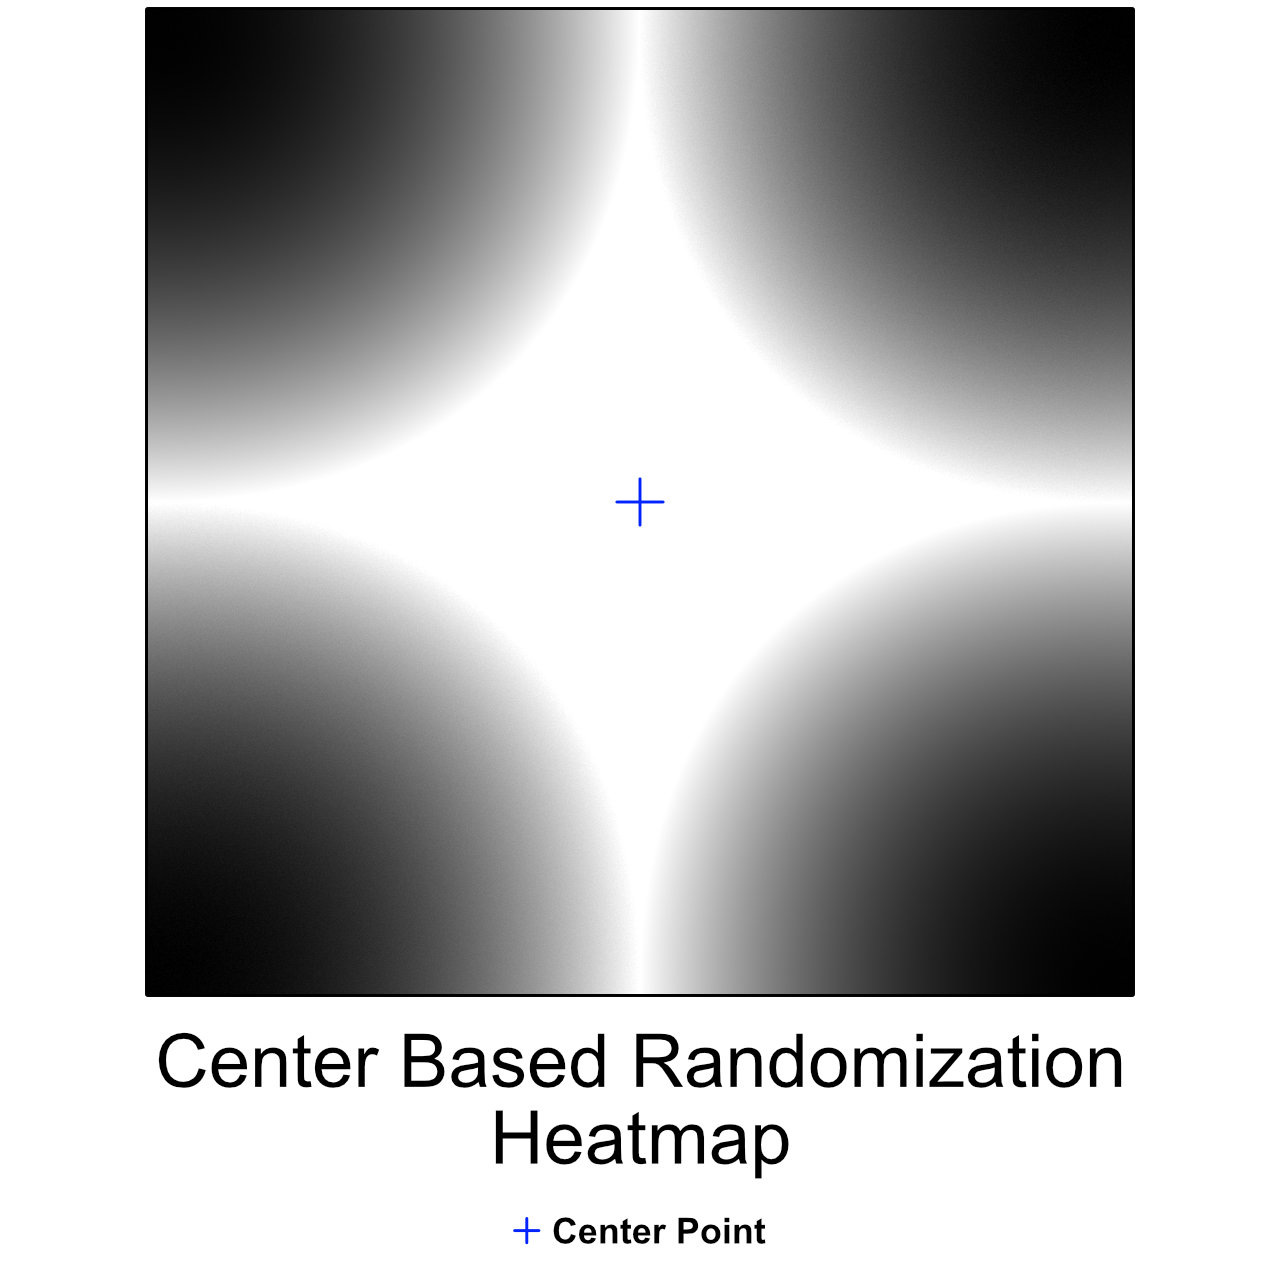
\includegraphics[width=0.65\textwidth]{img/cbr-map}
\caption{Heat map of a 2D area of points that are more likely to less likely to be generated from light to dark based on a center point}
\end{center}
\end{figure}

\par The points that are near to the axis of the center point are more likely to be generated than those that are far from the center point when the `deg' is greater than 1. When `deg' is less than 1, points far from the center point are generated more while when `deg' is 1, it is generating a uniform random number only.

\par The following figure shows generating random points using the mentioned technique with different centers and degree of nearness.

\begin{figure}
  \centering
  \begin{subfigure}[b]{0.4\textwidth}
    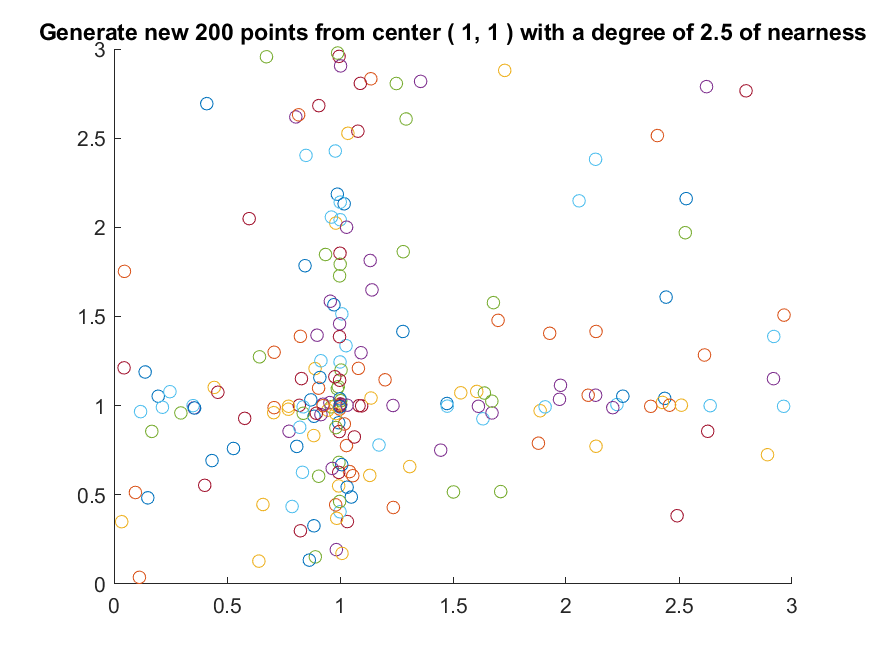
\includegraphics[width=\textwidth]{img/cbr-0}
    \label{fig:cbr-0}
  \end{subfigure}
  \begin{subfigure}[b]{0.4\textwidth}
    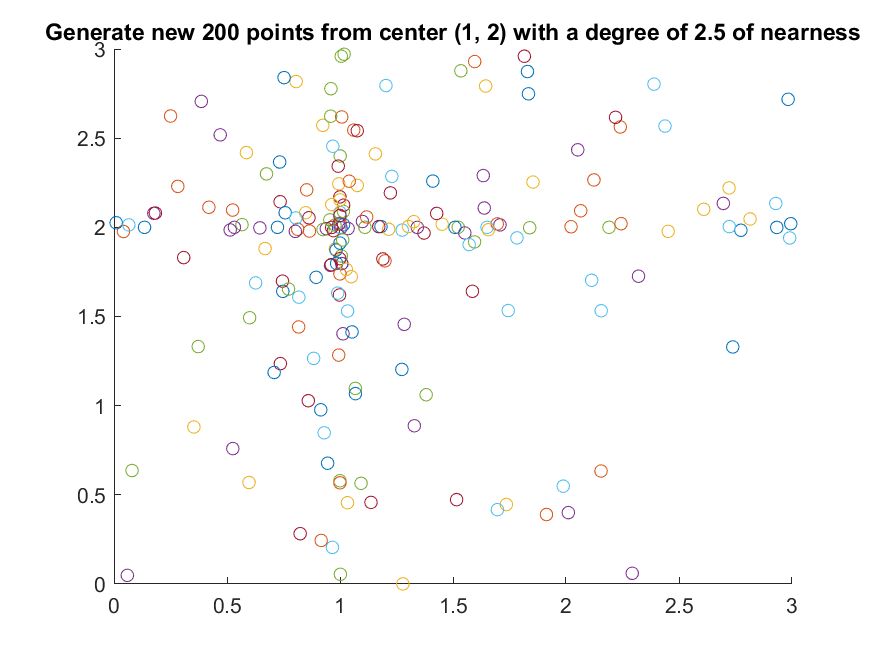
\includegraphics[width=\textwidth]{img/cbr-1}
    \label{fig:cbr-1}
  \end{subfigure}

  \begin{subfigure}[b]{0.4\textwidth}
    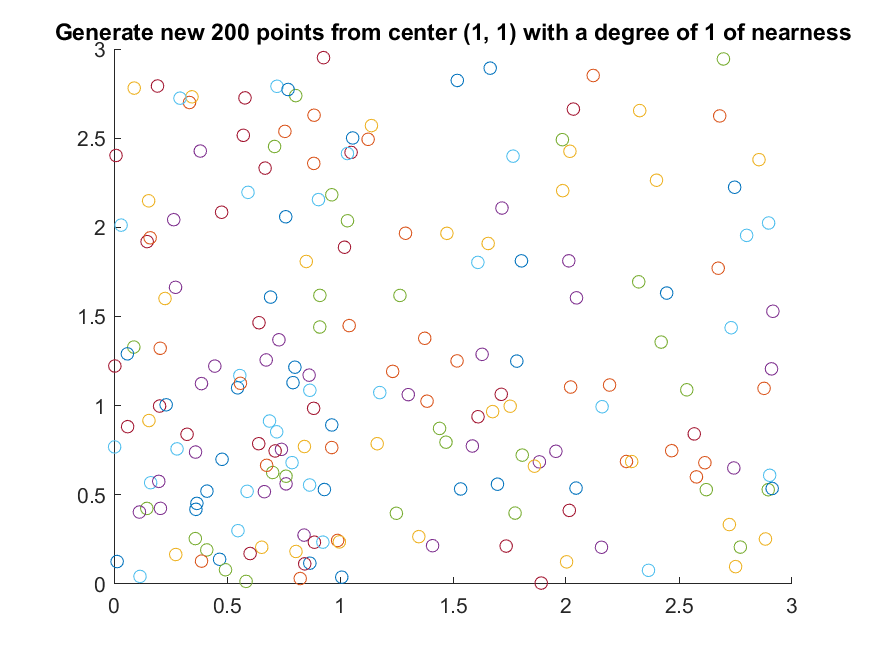
\includegraphics[width=\textwidth]{img/cbr-2}
    \label{fig:cbr-2}
  \end{subfigure}
  \begin{subfigure}[b]{0.4\textwidth}
    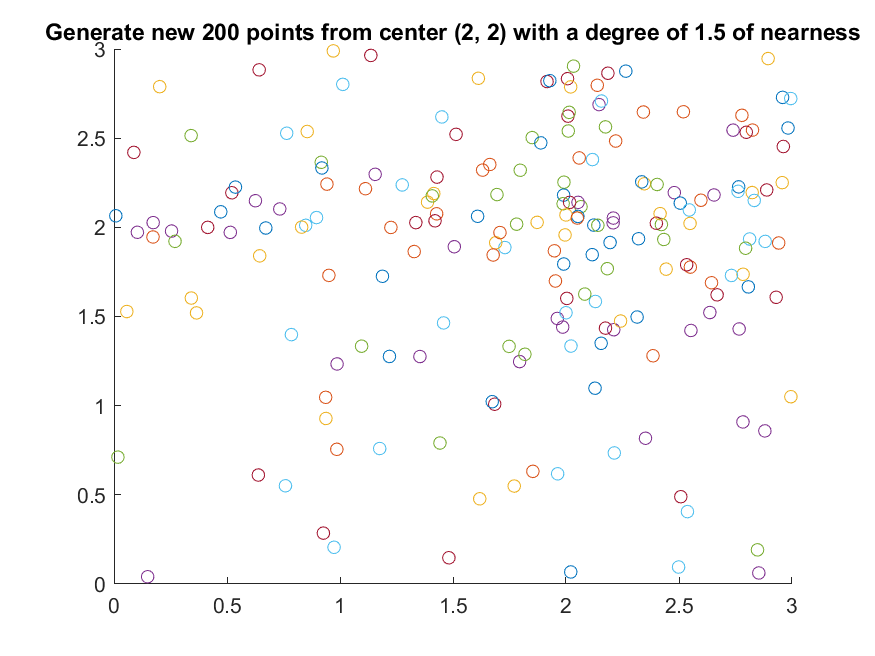
\includegraphics[width=\textwidth]{img/cbr-3}
    \label{fig:cbr-3}
  \end{subfigure}

  \begin{subfigure}[b]{0.4\textwidth}
    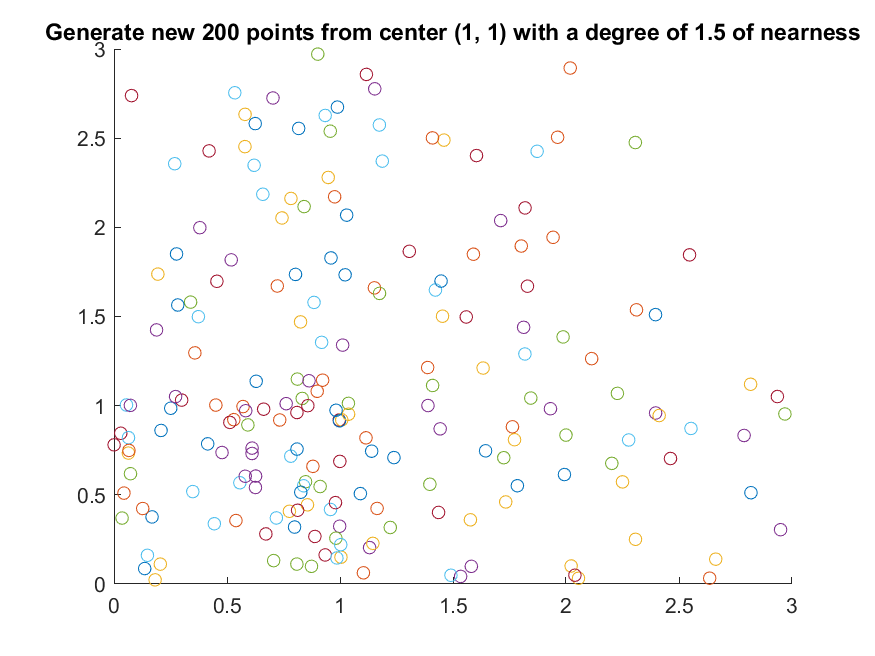
\includegraphics[width=\textwidth]{img/cbr-4}
    \label{fig:cbr-4}
  \end{subfigure}
  \begin{subfigure}[b]{0.4\textwidth}
    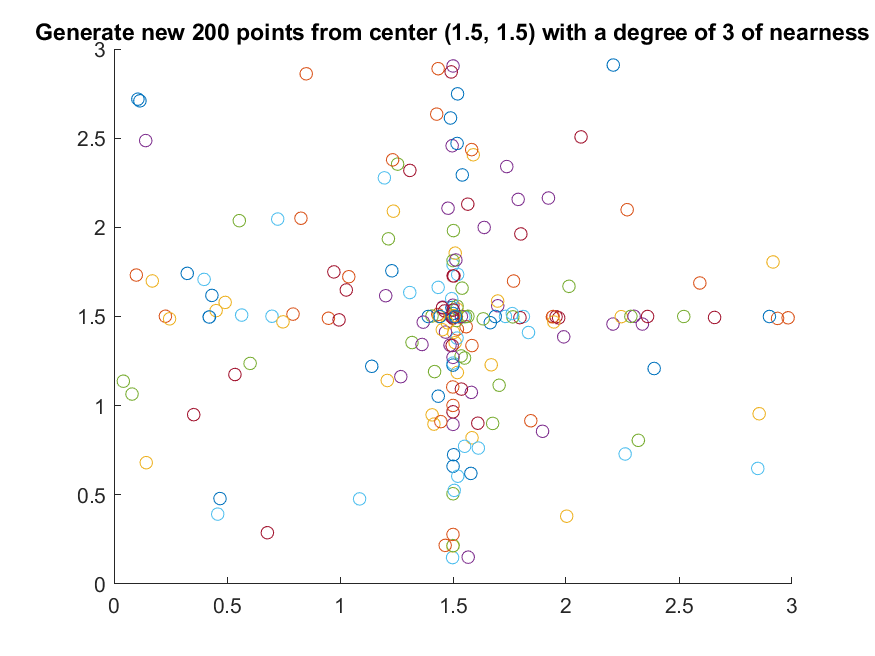
\includegraphics[width=\textwidth]{img/cbr-5}
    \label{fig:cbr-5}
  \end{subfigure}

  \begin{subfigure}[b]{0.4\textwidth}
    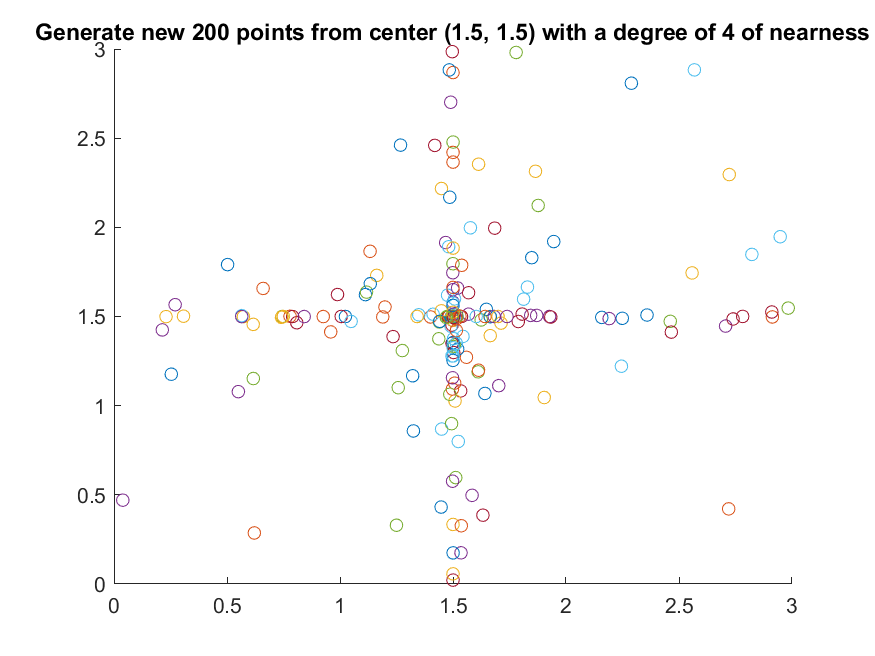
\includegraphics[width=\textwidth]{img/cbr-6}
    \label{fig:cbr-6}
  \end{subfigure}
  \begin{subfigure}[b]{0.4\textwidth}
    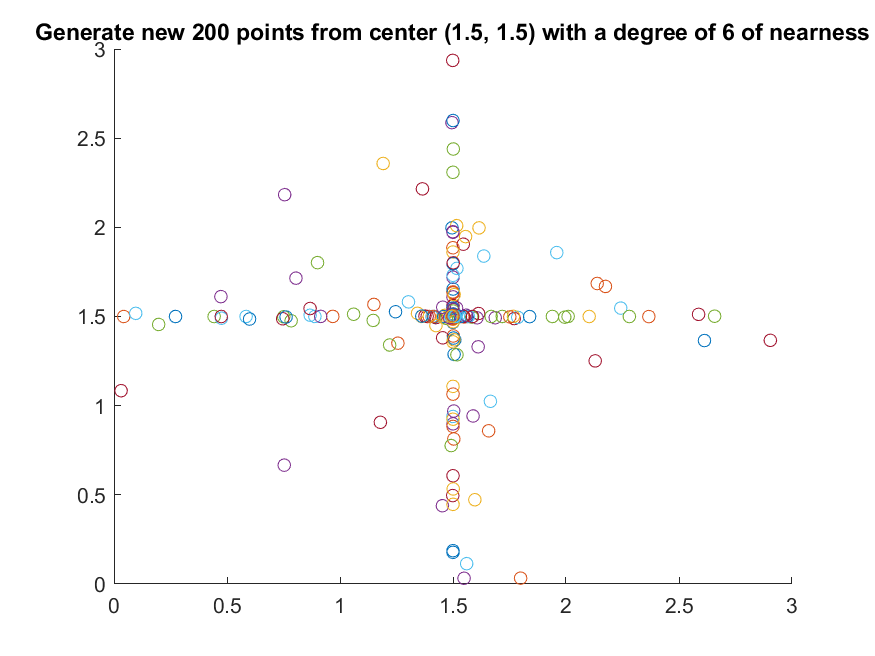
\includegraphics[width=\textwidth]{img/cbr-7}
    \label{fig:cbr-7}
  \end{subfigure}

  \caption{Center Based Random Points with Varying Centers and Nearness}
\end{figure}

\section{Modified Program Flow for the New Algorithm}

Combining together every improvement to the Lion Optimization Algorithm, the new flow of the new algorithm, that can be now called as the Improved Lion Optimization Algorithm (iLOA), is as follows:

\fbox{\begin{minipage}{0.9\textwidth}
\scriptsize

\textbf{Improved Lion Optimization Algorithm pseudo code}

\begin{enumerate}
  \item Generate random sample of Lions N$_{pop}$(N$_{pop}$ is number of initial population).
  \item Initiate prides and nomad lions
    \begin{itemize}
      \item Randomly select \%N (Percent of lions that are nomad) of initial population as nomad lion. Partition remained lions into P (P is number of prides) prides randomly, and formed each pride’s territory.
      \item In each pride \%S (Sex rate) of entire population are known as females and the rest as males. This rate in nomad lions is inversed.
    \end{itemize}
  \item For each pride do
    \begin{itemize}
      \item Some randomly selected female lion go hunting.
      \item Each of remained female lion in pride go toward one place in the territory selected randomly but with bias to the better places (Ranked Selection Random). The direction of each female would be influenced by the direction to the best place in the territory by \%I (Group Influence)
      \item In pride, for each resident male; \%R (Roaming percent) of territory randomly are selected with bias to the better places (Ranked Selection Random) and then checked with the influence of the best place in the territory by \%I (Group Influence).
      \item \%Ma (Mating probability) of females with bias to the best females (Ranked Selection Random) in pride mate with one or several resident male. The stronger the male lion’s gene, the better it influences the offspring (Fitness Weighted Mating). — New cubs become mature.
      \item Weakest male drive out from pride and checked whether it is within the lower bound fitness of nomads.
      \begin{itemize}
        \item Joins nomads, otherwise, killed (Simulated Annealing)
      \end{itemize}
    \end{itemize}
  \item For Nomad do
    \begin{itemize}
      \item Nomad lion (both male and female) moving randomly in search space. Every random is centered on the best nomad lion in the group and biased near it (Center Based Randomization).
      \item \%Ma (Mating probability) of nomad Female mate with one of the best nomad male. — New cubs become mature.
      \item Prides randomly attacked by nomad male.
    \end{itemize}
  \item For each pride do
    \begin{itemize}
      \item Some female with I rate ((Immigrate rate)) immigrate from pride and become nomad.
    \end{itemize}
  \item Do
    \begin{itemize}
      \item First, based on their fitness value each gender of the nomad lions are sorted. After that, the best females among them are selected and distributed to prides filling empty places of migrated females.
      \item With respect to the maximum permitted number of each gender, nomad lions with the least fitness value will be removed.
    \end{itemize}
\end{enumerate}
If termination criterion is not satisfied, then go to step c
\end{minipage}}

\section{Testing against LOA}
\par Both algorithms are tested head to head through various benchmarking functions which includes: Griewank 1D and 2D, Rastrigin 1D and 2D, Rosenbrock 2D, Parabola and Paraboloid. Each function use different dimensional space but all run for 50 iterations with 50 population and the following parameters:

\fbox{\begin{minipage}{0.9\textwidth}
\scriptsize
\textbf{Number of Prides} = 4 \\
\textbf{Nomad Percentage (\%N)} = 0.2 \\
\textbf{Roaming Percentage (\%R)} = 0.2 \\
\textbf{Sex Percentage (\%S)} = 0.8 \\
\textbf{Mating Rate (\%Ma)} = 0.3 \\
\textbf{Mutation Probability} = 0.2 \\
\textbf{Immigration Rate} = 0.4 \\
-- More parameters for iLOA -- \\
\textbf{Percent Group Influence} = 0.4 \\
\textbf{Annealing} = True \\
\textbf{Ranked Selection Pressure} = 2 \\
\textbf{Near to Best Random Pressure} = 2
\end{minipage}}

\subsection{Griewank 1D}

\par The Griewank function is a function that is typically used for testing optimization. The function is defined by:

$$
f_1(x) = 1+(1/4000)\cdot x_1^2-\cos(x_1)
$$

It has multiple maxima and minima but its global minima is at $x=0$.

\par Both functions are tested five times with the Griewank function with the same starting random population and a dimensional space of [-100, 100].

\begin{table}[ht]
\scriptsize
\begin{tabular}{l|ccccc}
\textbf{}        & \textbf{Trial 1} & \textbf{Trial 2} & \textbf{Trial 3} & \textbf{Trial 4} & \textbf{Trial 5} \\
\hline
LOA End Fitness  & 1.5846E-07       & 1.2658E-07       & 7.4251E-08       & 3.5575E-06       & 5.4992E-08       \\
LOA Evaluations  & 3499             & 3453             & 3465             & 3560             & 3468             \\
iLOA End Fitness & 9.3769E-10       & 3.1541E-13       & 4.5715E-11       & 1.8532E-09       & 2.1836E-12       \\
iLOA Evaluations & 3042             & 2803             & 2710             & 2718             & 2857
\end{tabular}
\caption{ \scriptsize LOA vs. iLOA: Griewank 1D ($f_1$)}
\end{table}

\begin{figure}
  \centering
  \begin{subfigure}[b]{0.4\textwidth}
    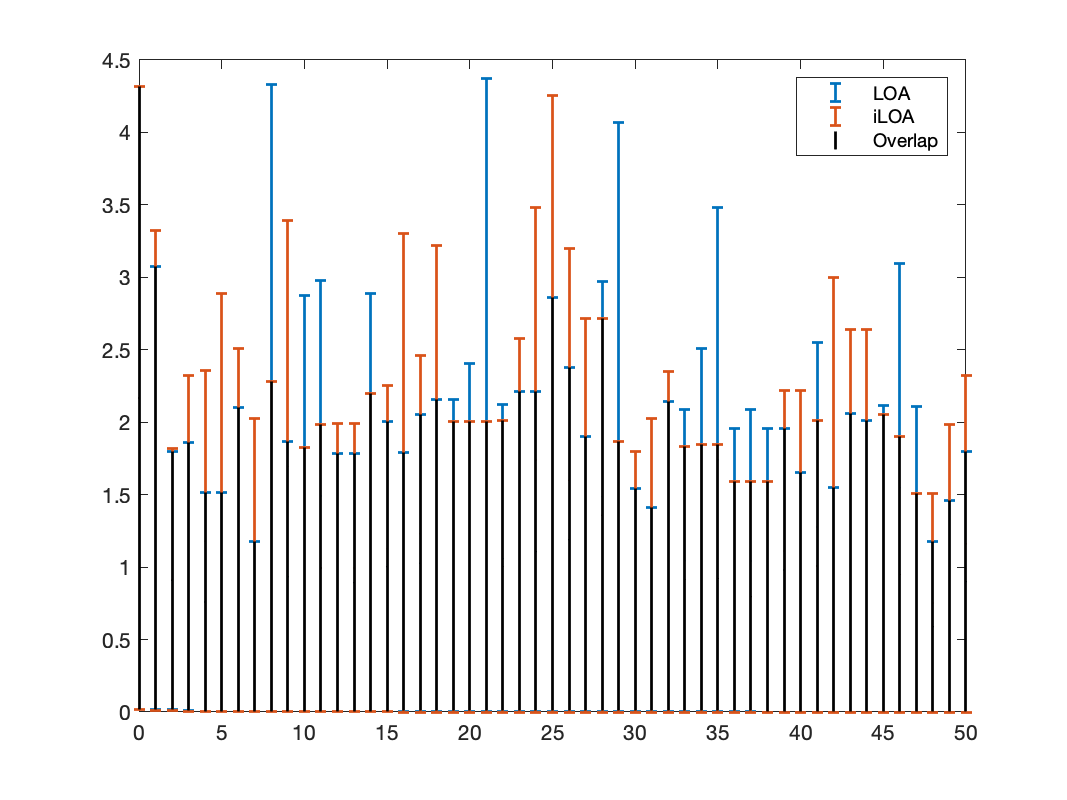
\includegraphics[width=\textwidth]{img/bars/f1/1}
    \caption{ \scriptsize Trial 1: Fitness Range (y) over Iterations (x)}
    \label{fig:f1-b-1}
  \end{subfigure}
  \begin{subfigure}[b]{0.4\textwidth}
    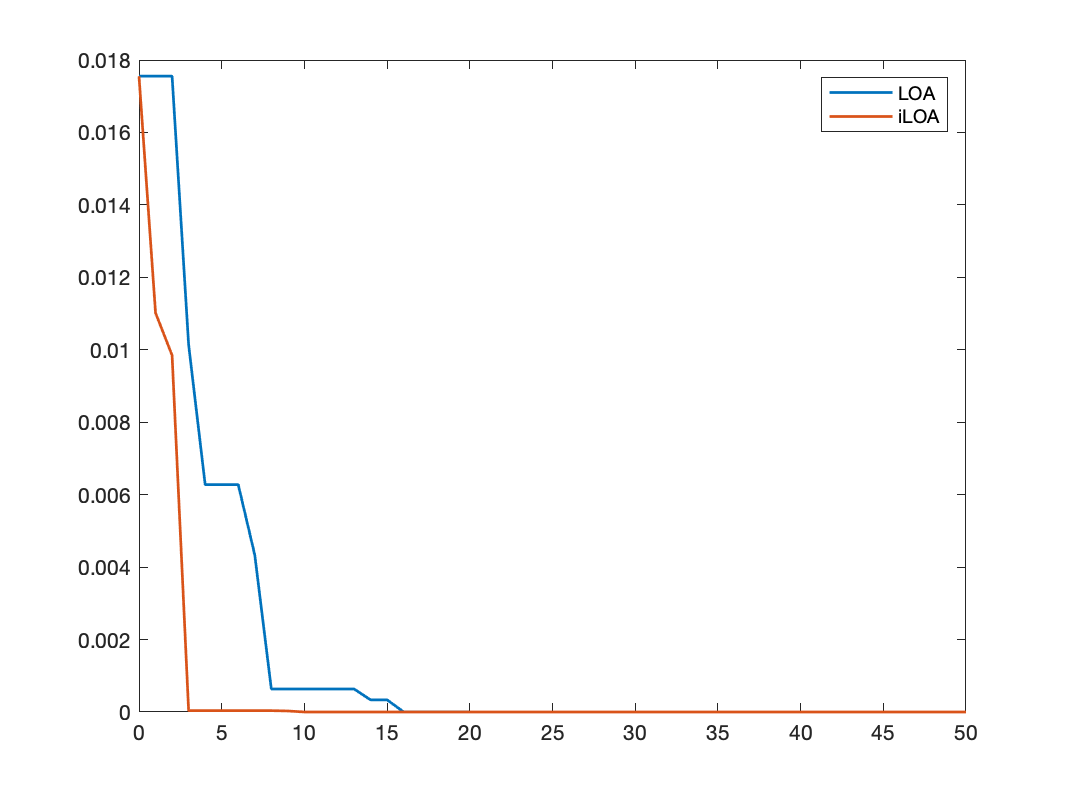
\includegraphics[width=\textwidth]{img/fits/f1/1}
    \caption{ \scriptsize Trial 1: Minimum Fitness (y) over Iterations (x)}
    \label{fig:f1-f-1}
  \end{subfigure}

  \begin{subfigure}[b]{0.4\textwidth}
    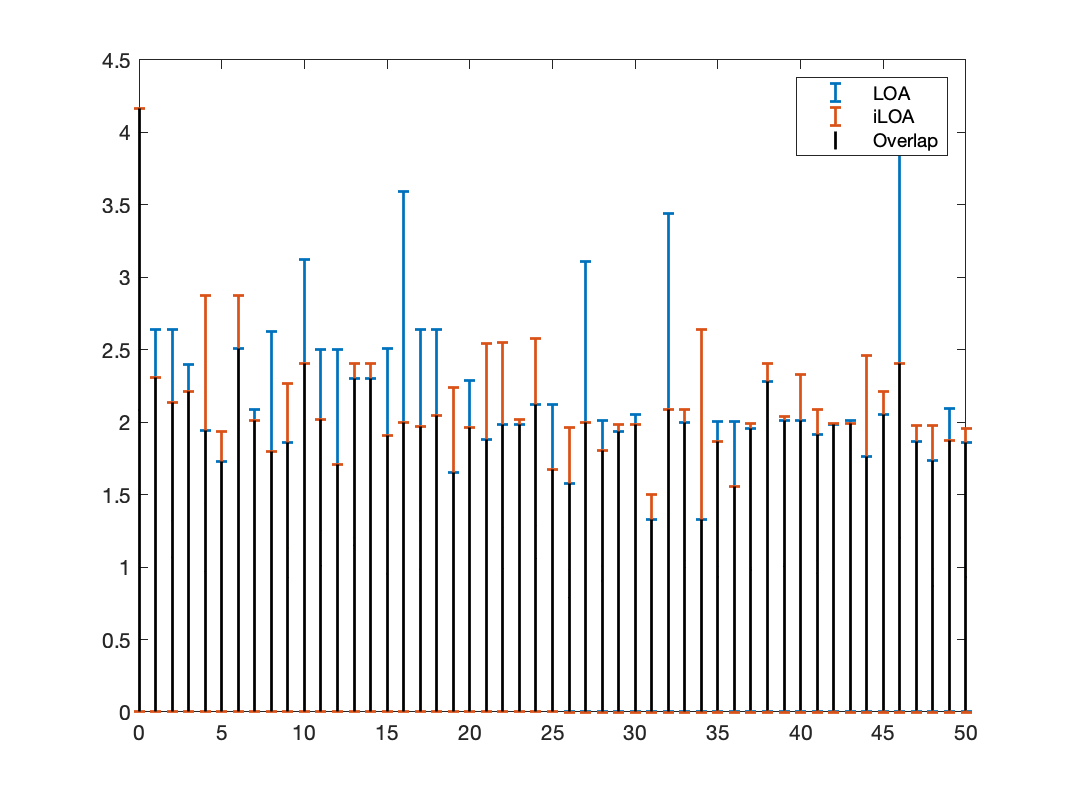
\includegraphics[width=\textwidth]{img/bars/f1/2}
    \caption{ \scriptsize Trial 2: Fitness Range (y) over Iterations (x)}
    \label{fig:f1-b-2}
  \end{subfigure}
  \begin{subfigure}[b]{0.4\textwidth}
    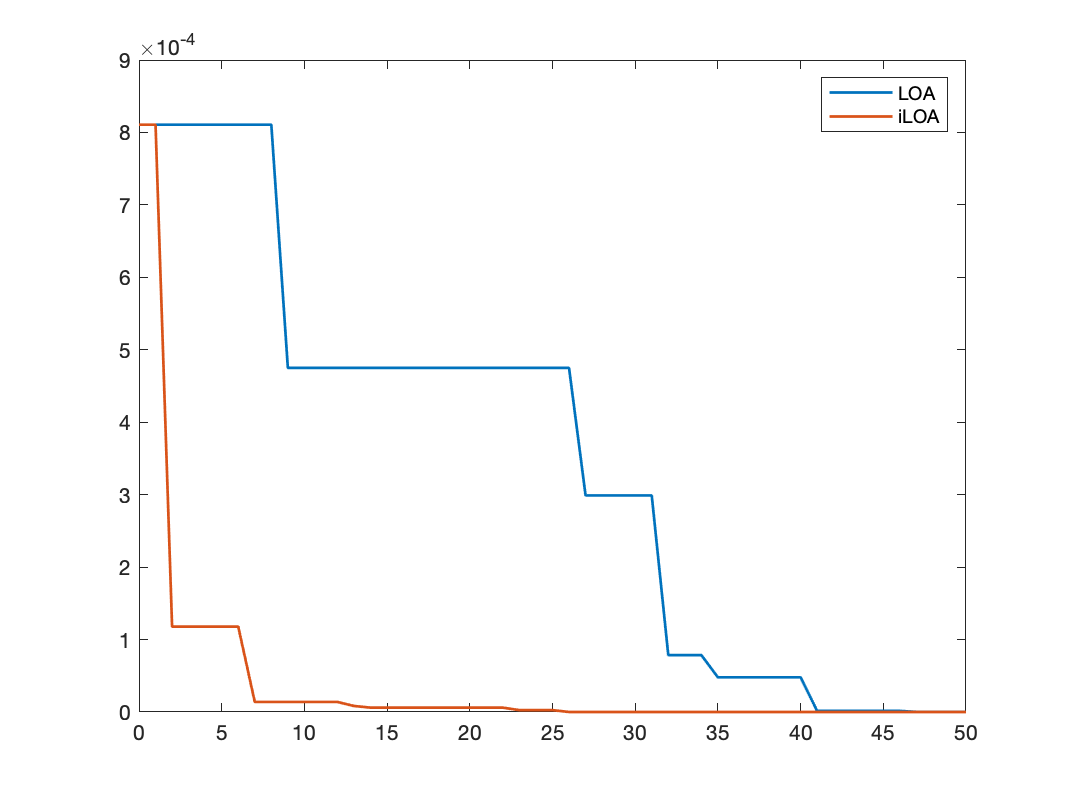
\includegraphics[width=\textwidth]{img/fits/f1/2}
    \caption{ \scriptsize Trial 2: Minimum Fitness (y) over Iterations (x)}
    \label{fig:f1-f-2}
  \end{subfigure}

  \begin{subfigure}[b]{0.4\textwidth}
    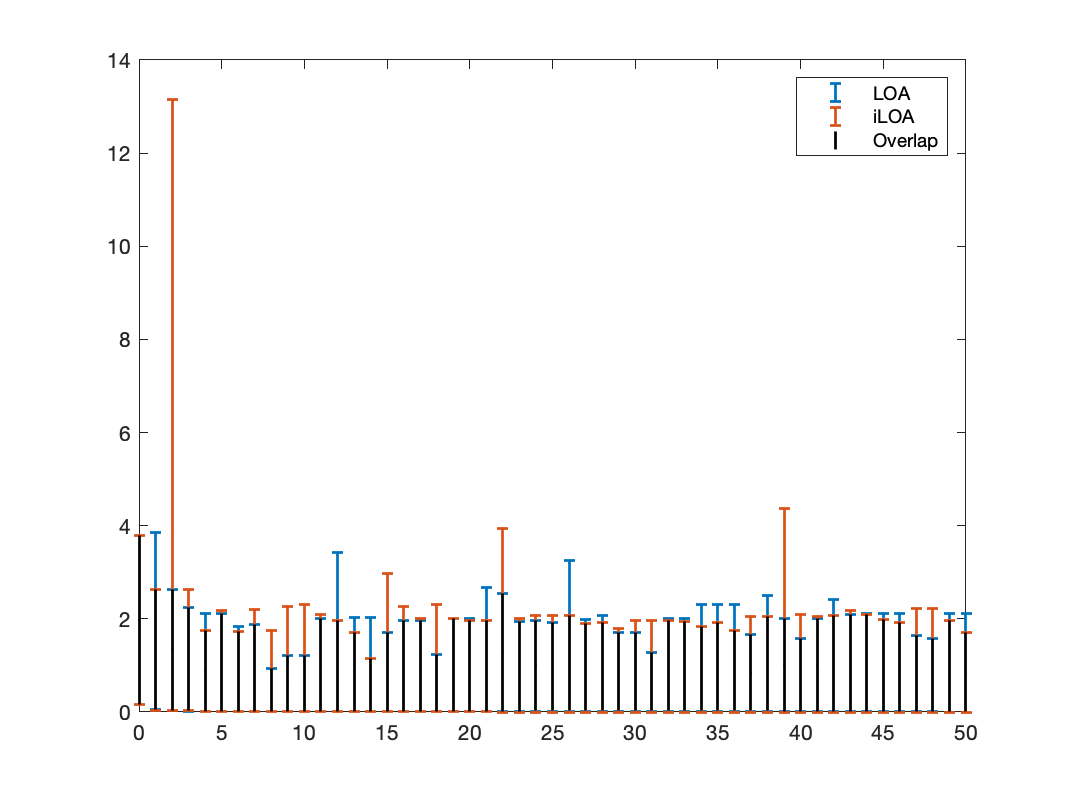
\includegraphics[width=\textwidth]{img/bars/f1/3}
    \caption{ \scriptsize Trial 3: Fitness Range (y) over Iterations (x)}
    \label{fig:f1-b-3}
  \end{subfigure}
  \begin{subfigure}[b]{0.4\textwidth}
    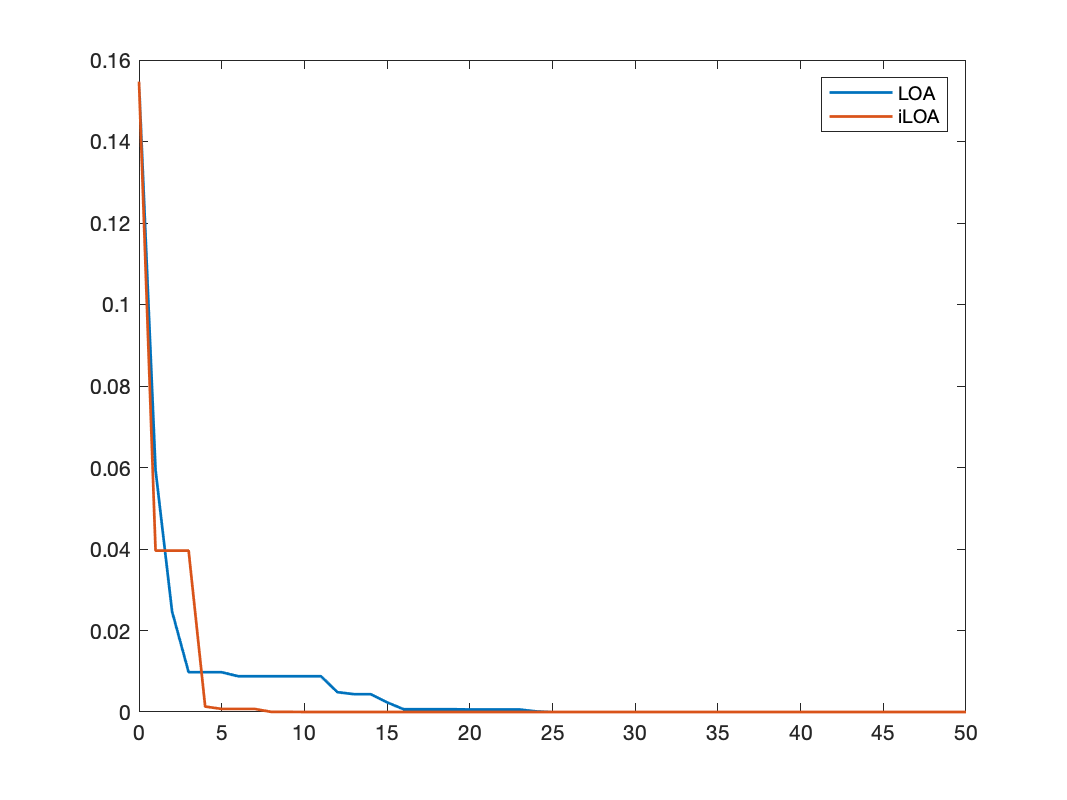
\includegraphics[width=\textwidth]{img/fits/f1/3}
    \caption{ \scriptsize Trial 3: Minimum Fitness (y) over Iterations (x)}
    \label{fig:f1-f-3}
  \end{subfigure}

  \begin{subfigure}[b]{0.4\textwidth}
    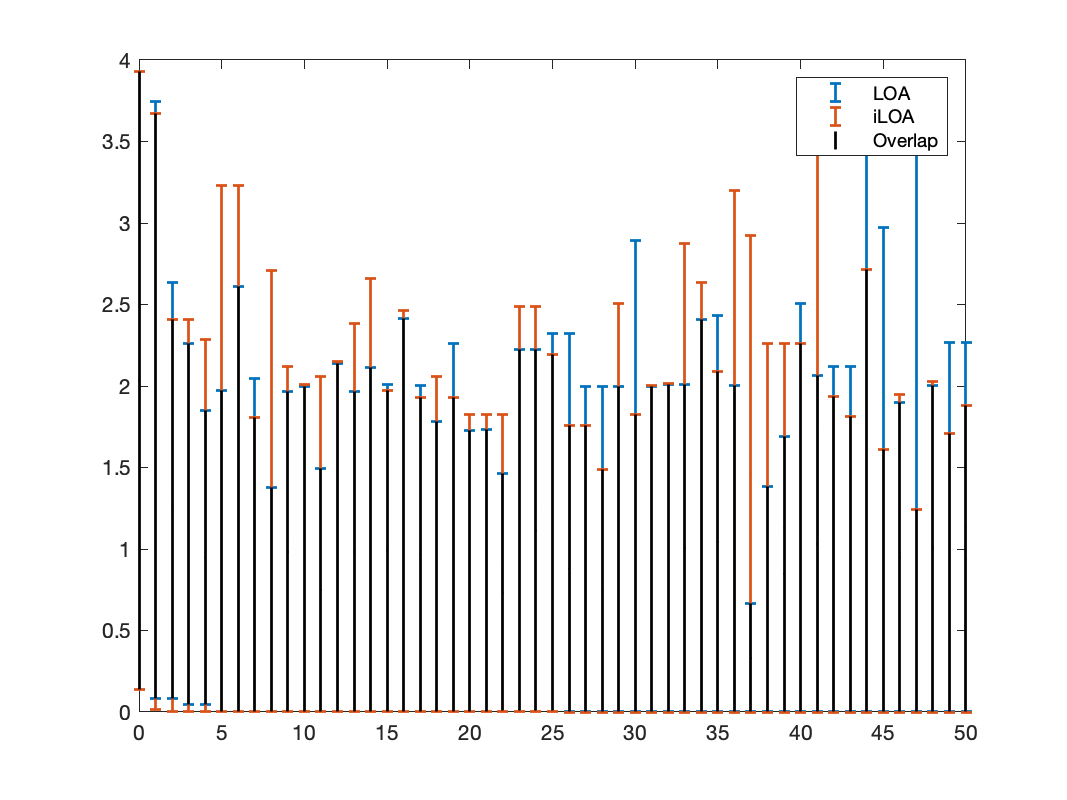
\includegraphics[width=\textwidth]{img/bars/f1/4}
    \caption{ \scriptsize Trial 4: Fitness Range (y) over Iterations (x)}
    \label{fig:f1-b-4}
  \end{subfigure}
  \begin{subfigure}[b]{0.4\textwidth}
    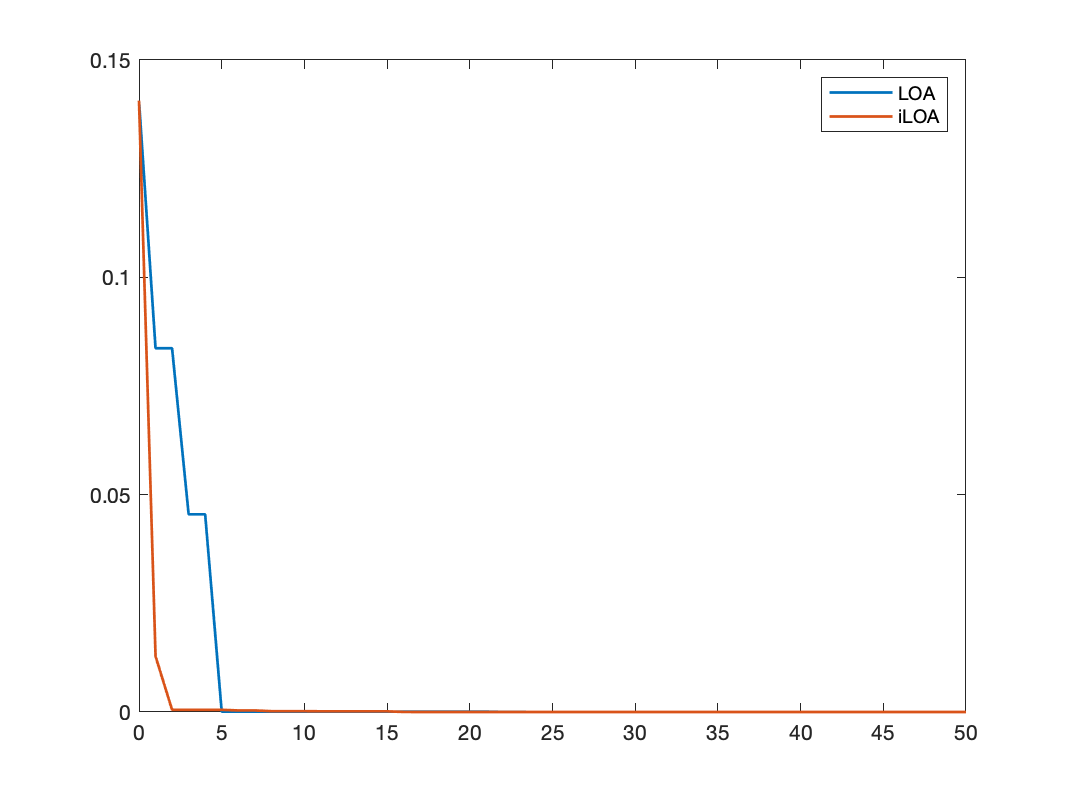
\includegraphics[width=\textwidth]{img/fits/f1/4}
    \caption{ \scriptsize Trial 4: Minimum Fitness (y) over Iterations (x)}
    \label{fig:f1-f-4}
  \end{subfigure}

  \begin{subfigure}[b]{0.4\textwidth}
    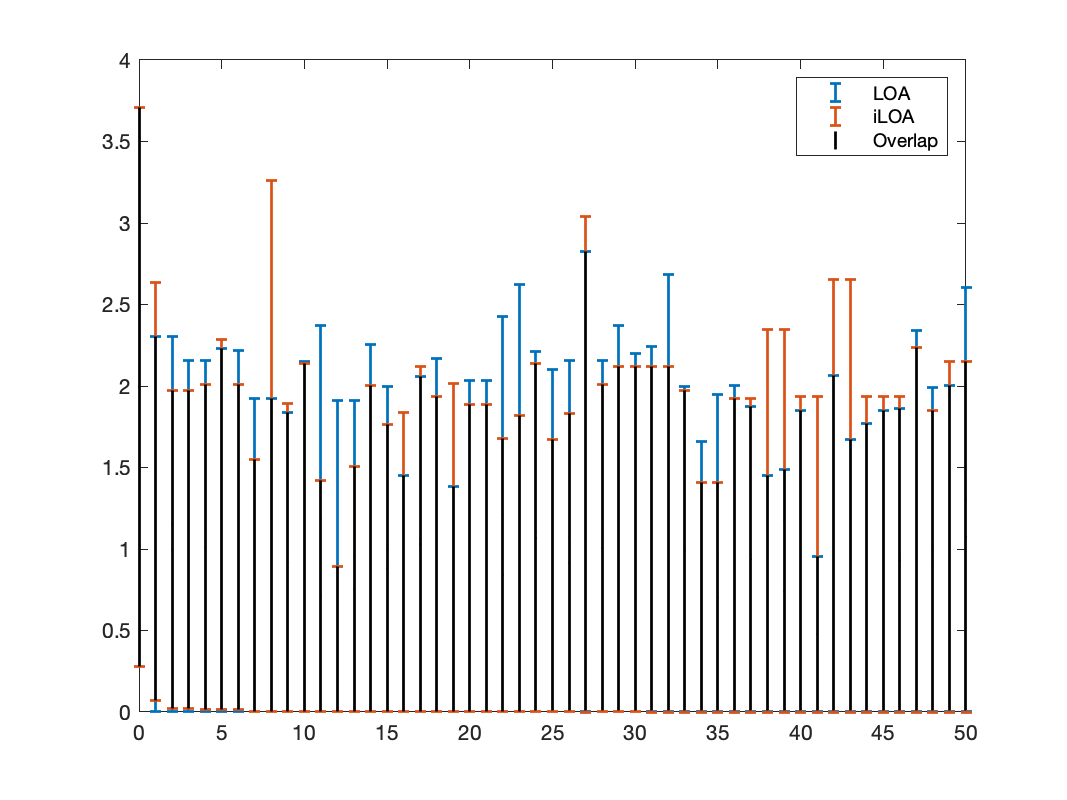
\includegraphics[width=\textwidth]{img/bars/f1/5}
    \caption{ \scriptsize Trial 5: Fitness Range (y) over Iterations (x)}
    \label{fig:f1-b-5}
  \end{subfigure}
  \begin{subfigure}[b]{0.4\textwidth}
    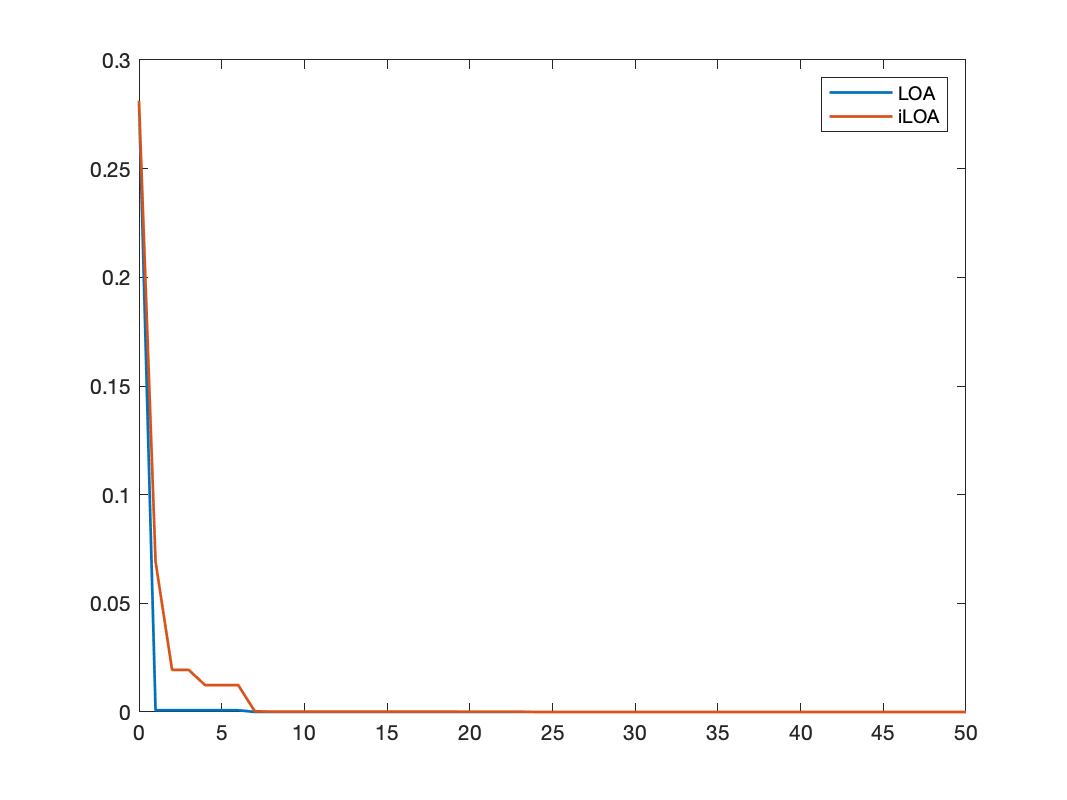
\includegraphics[width=\textwidth]{img/fits/f1/5}
    \caption{ \scriptsize Trial 5: Minimum Fitness (y) over Iterations (x)}
    \label{fig:f1-f-5}
  \end{subfigure}

  \caption{ \scriptsize LOA vs. iLOA: Griewank 1D ($f_1$)}
\end{figure}

\subsection{Griewank 2D}

\par The 2 dimensional form of the Griewank is the Griewank 2D function. The function is defined by:

$$
f_2(x) = 1+\frac {1}{4000} x_1^2 + \frac {1}{4000} x_2^2- \cos(x_1) \cos \left( \frac 1 2 x_2\sqrt {2} \right)
$$

It also has multiple maxima and minima and its global minima is also at $x=0$.

\par Both functions are tested five times with the Griewank 2D function with the same starting random population and a dimensional space of [-100, 100].

\begin{table}[ht]
\scriptsize
\begin{tabular}{l|ccccc}
\textbf{}        & \textbf{Trial 1} & \textbf{Trial 2} & \textbf{Trial 3} & \textbf{Trial 4} & \textbf{Trial 5} \\
\hline
LOA End Fitness  & 0.0091998        & 0.010329         & 0.0069254        & 0.0010238        & 0.01839          \\
LOA Evaluations  & 3440             & 3468             & 3508             & 3525             & 3476             \\
iLOA End Fitness & 0.011425         & 0.00038845       & 0.00004408       & 0.00011175       & 0.011947         \\
iLOA Evaluations & 2609             & 2588             & 2705             & 2554             & 2649
\end{tabular}
\caption{ \scriptsize LOA vs. iLOA: Griewank 2D ($f_2$)}
\end{table}

\begin{figure}
  \centering
  \begin{subfigure}[b]{0.4\textwidth}
    \includegraphics[width=\textwidth]{img/bars/f2/1}
    \caption{ \scriptsize Trial 1: Fitness Range (y) over Iterations (x)}
    \label{fig:f2-b-1}
  \end{subfigure}
  \begin{subfigure}[b]{0.4\textwidth}
    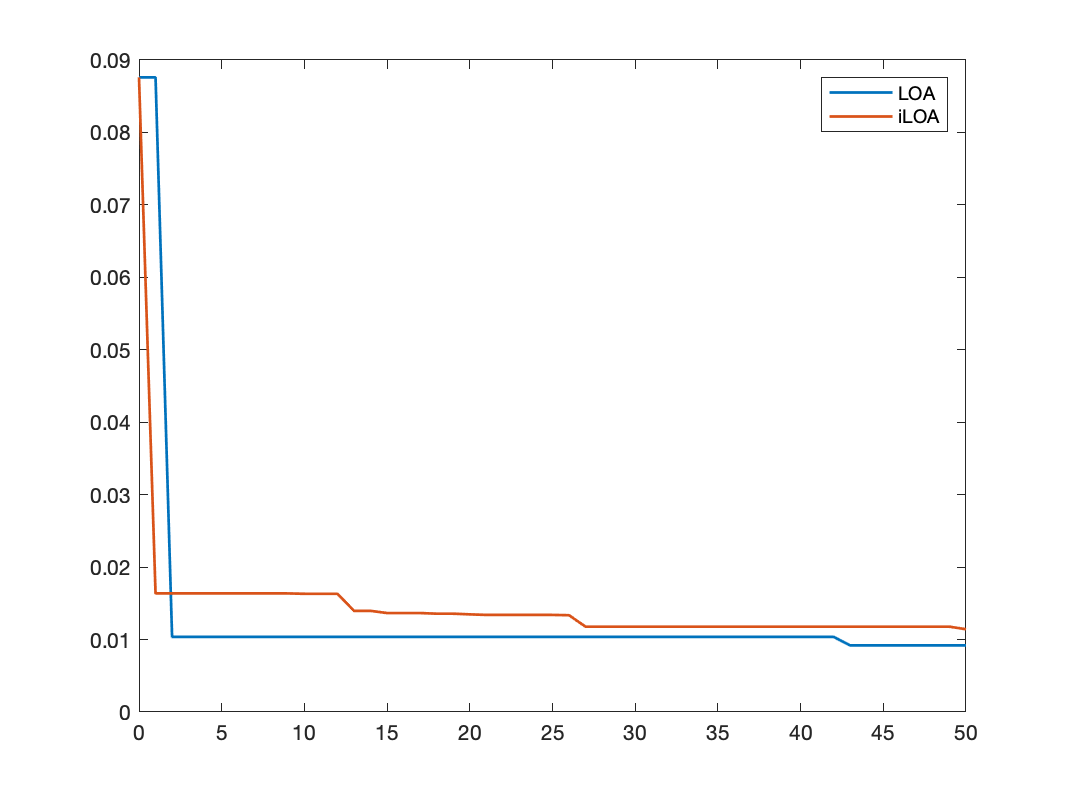
\includegraphics[width=\textwidth]{img/fits/f2/1}
    \caption{ \scriptsize Trial 1: Minimum Fitness (y) over Iterations (x)}
    \label{fig:f2-f-1}
  \end{subfigure}

  \begin{subfigure}[b]{0.4\textwidth}
    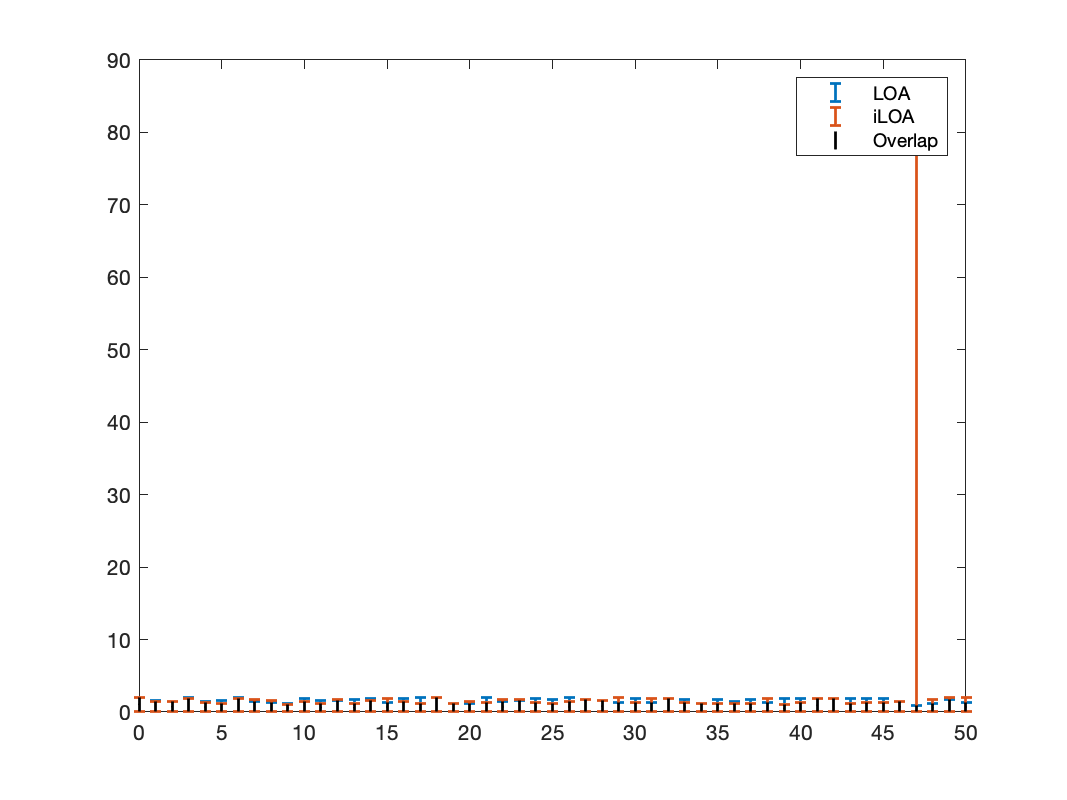
\includegraphics[width=\textwidth]{img/bars/f2/2}
    \caption{ \scriptsize Trial 2: Fitness Range (y) over Iterations (x)}
    \label{fig:f2-b-2}
  \end{subfigure}
  \begin{subfigure}[b]{0.4\textwidth}
    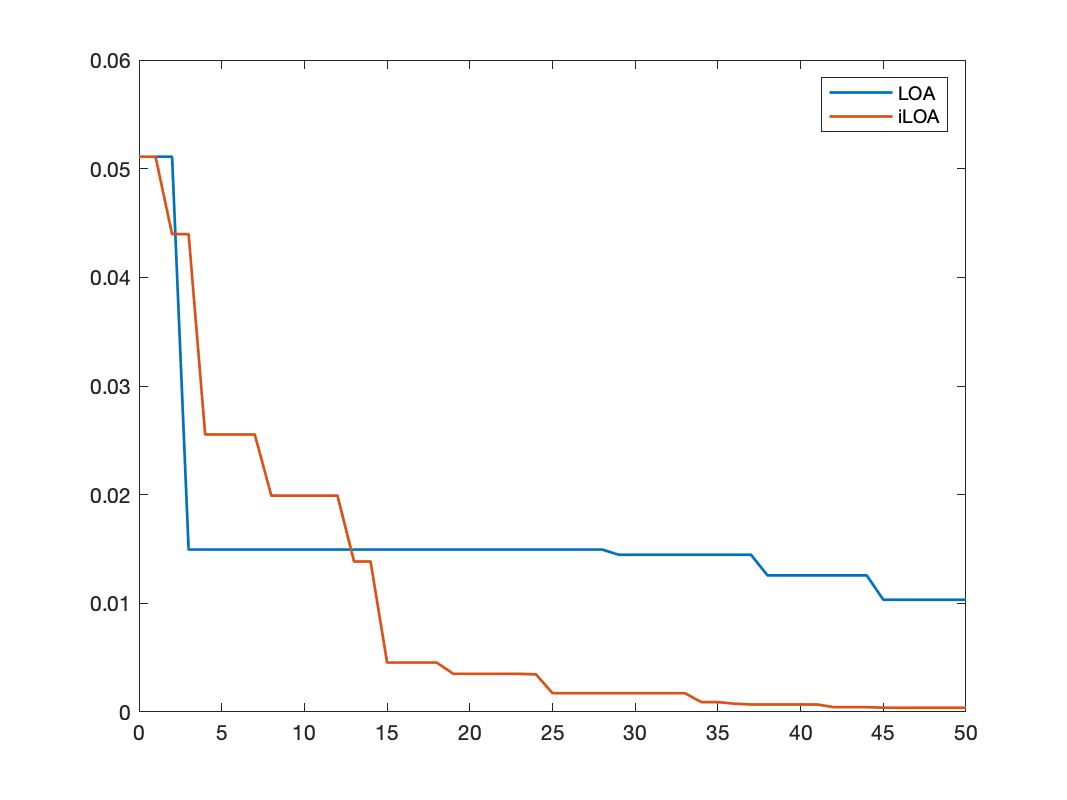
\includegraphics[width=\textwidth]{img/fits/f2/2}
    \caption{ \scriptsize Trial 2: Minimum Fitness (y) over Iterations (x)}
    \label{fig:f2-f-2}
  \end{subfigure}

  \begin{subfigure}[b]{0.4\textwidth}
    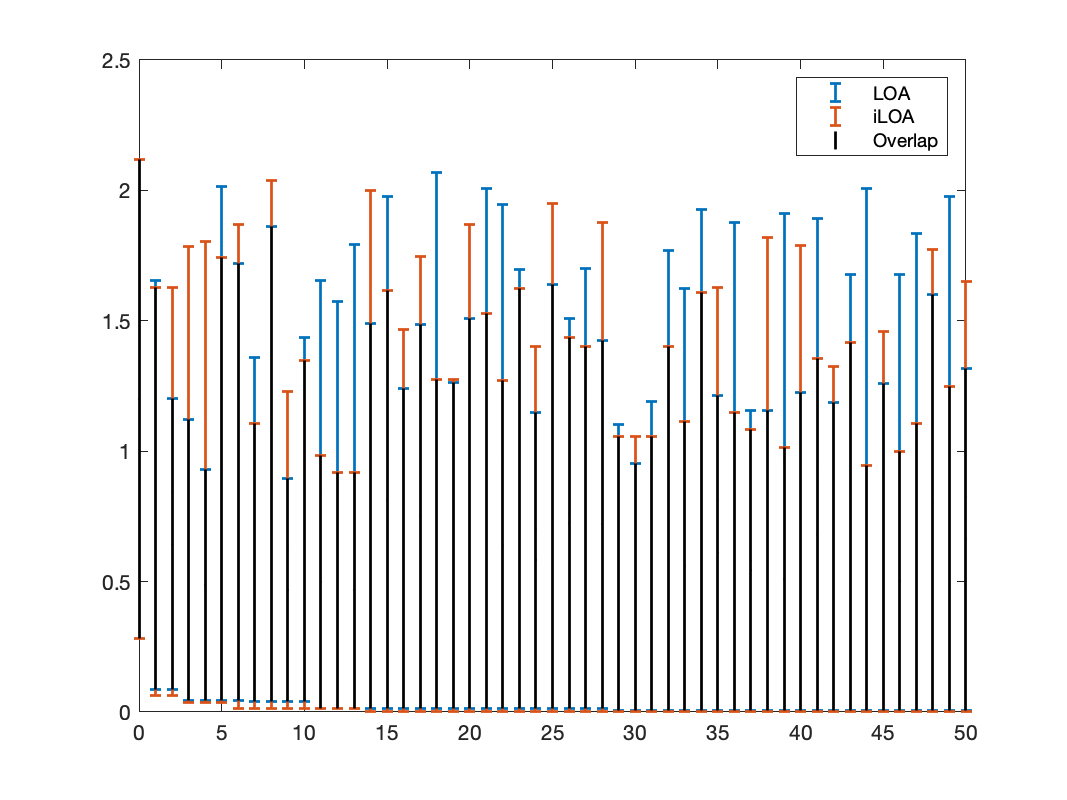
\includegraphics[width=\textwidth]{img/bars/f2/3}
    \caption{ \scriptsize Trial 3: Fitness Range (y) over Iterations (x)}
    \label{fig:f2-b-3}
  \end{subfigure}
  \begin{subfigure}[b]{0.4\textwidth}
    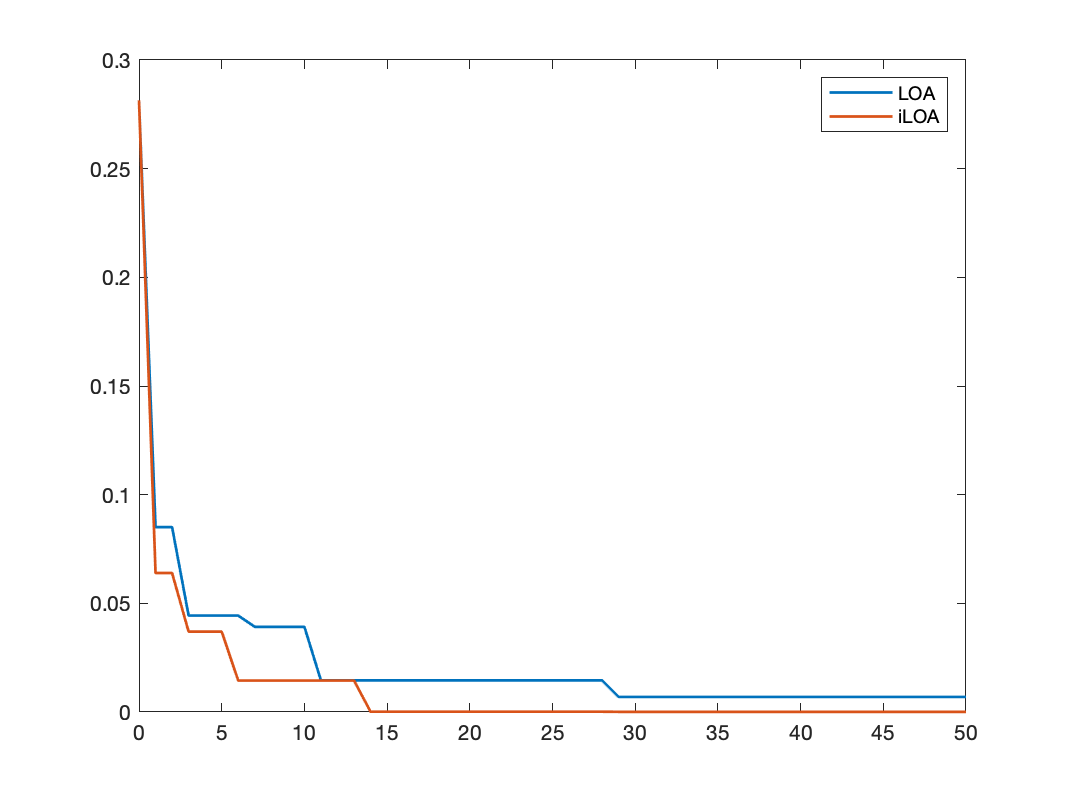
\includegraphics[width=\textwidth]{img/fits/f2/3}
    \caption{ \scriptsize Trial 3: Minimum Fitness (y) over Iterations (x)}
    \label{fig:f2-f-3}
  \end{subfigure}

  \begin{subfigure}[b]{0.4\textwidth}
    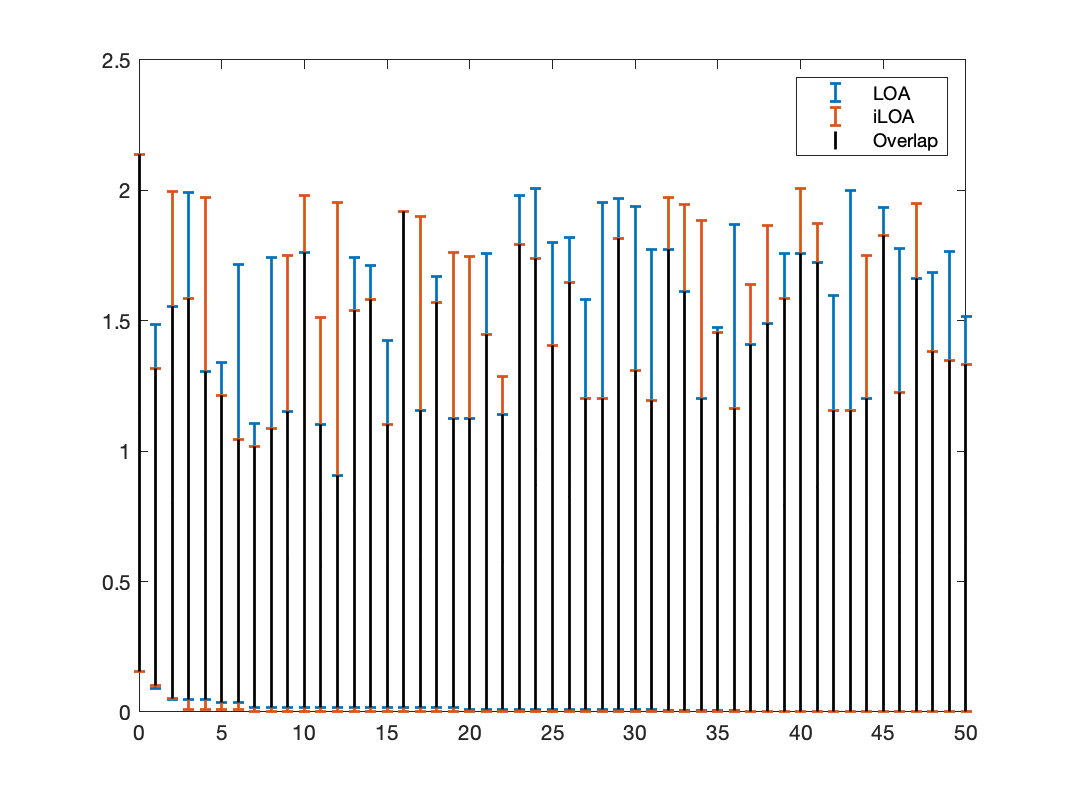
\includegraphics[width=\textwidth]{img/bars/f2/4}
    \caption{ \scriptsize Trial 4: Fitness Range (y) over Iterations (x)}
    \label{fig:f2-b-4}
  \end{subfigure}
  \begin{subfigure}[b]{0.4\textwidth}
    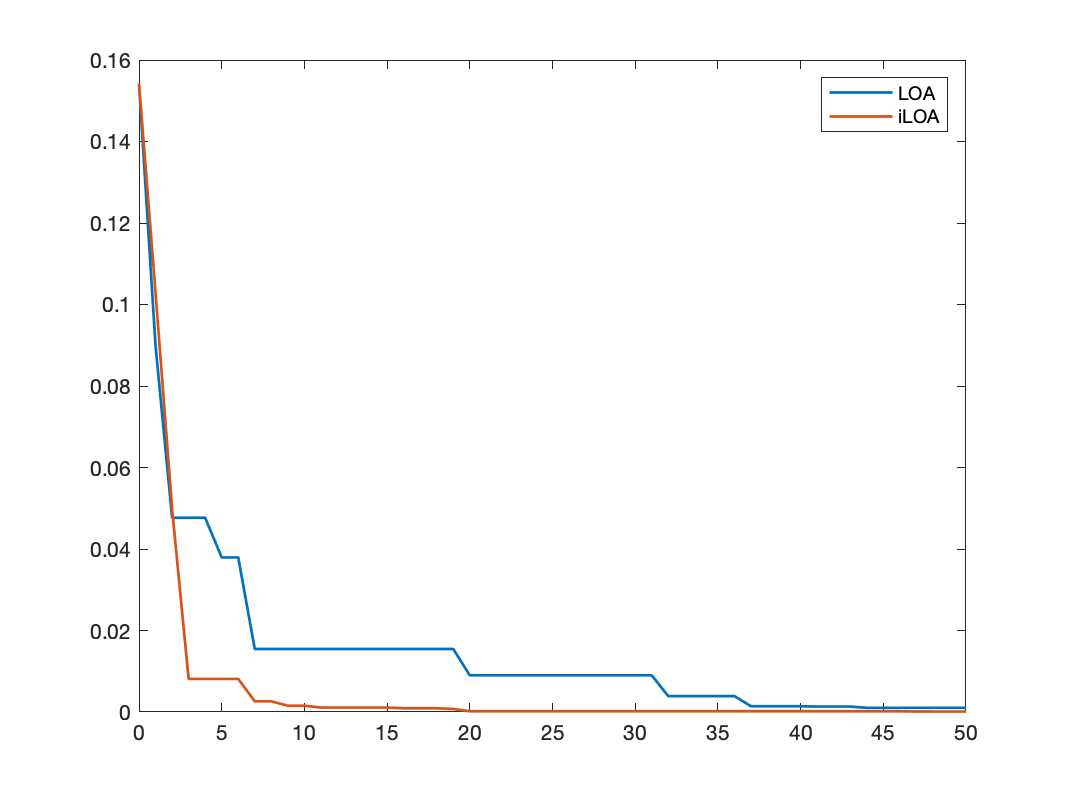
\includegraphics[width=\textwidth]{img/fits/f2/4}
    \caption{ \scriptsize Trial 4: Minimum Fitness (y) over Iterations (x)}
    \label{fig:f2-f-4}
  \end{subfigure}

  \begin{subfigure}[b]{0.4\textwidth}
    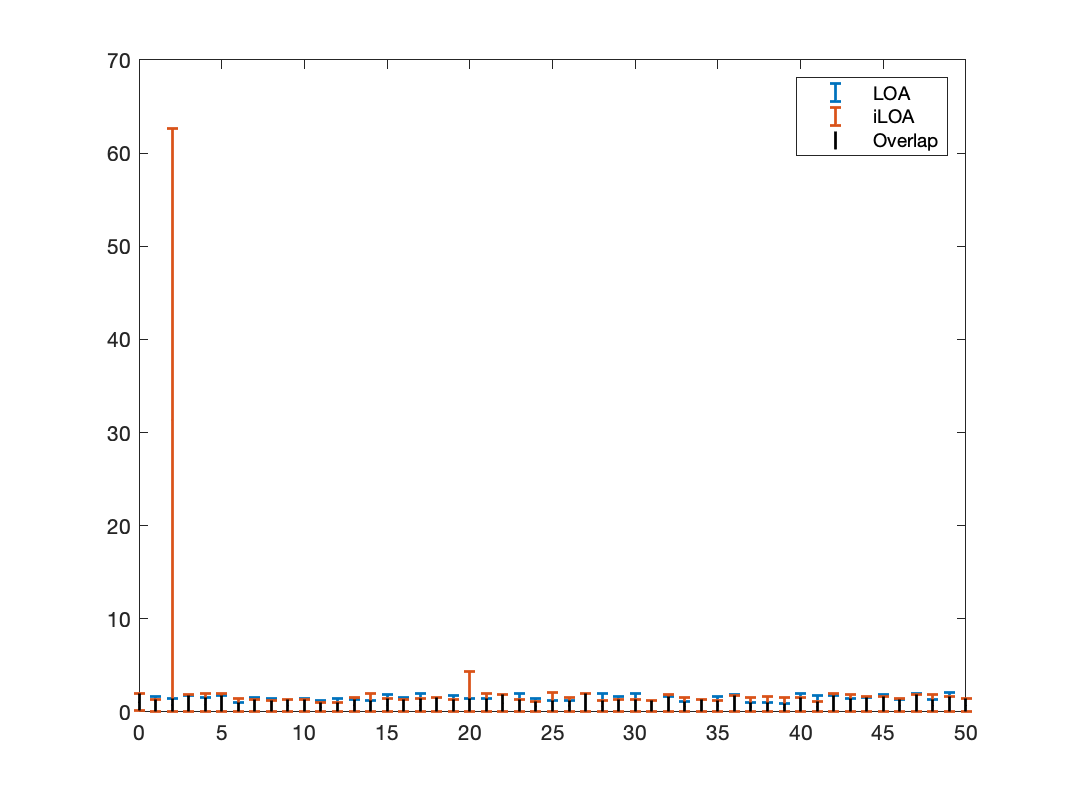
\includegraphics[width=\textwidth]{img/bars/f2/5}
    \caption{ \scriptsize Trial 5: Fitness Range (y) over Iterations (x)}
    \label{fig:f2-b-5}
  \end{subfigure}
  \begin{subfigure}[b]{0.4\textwidth}
    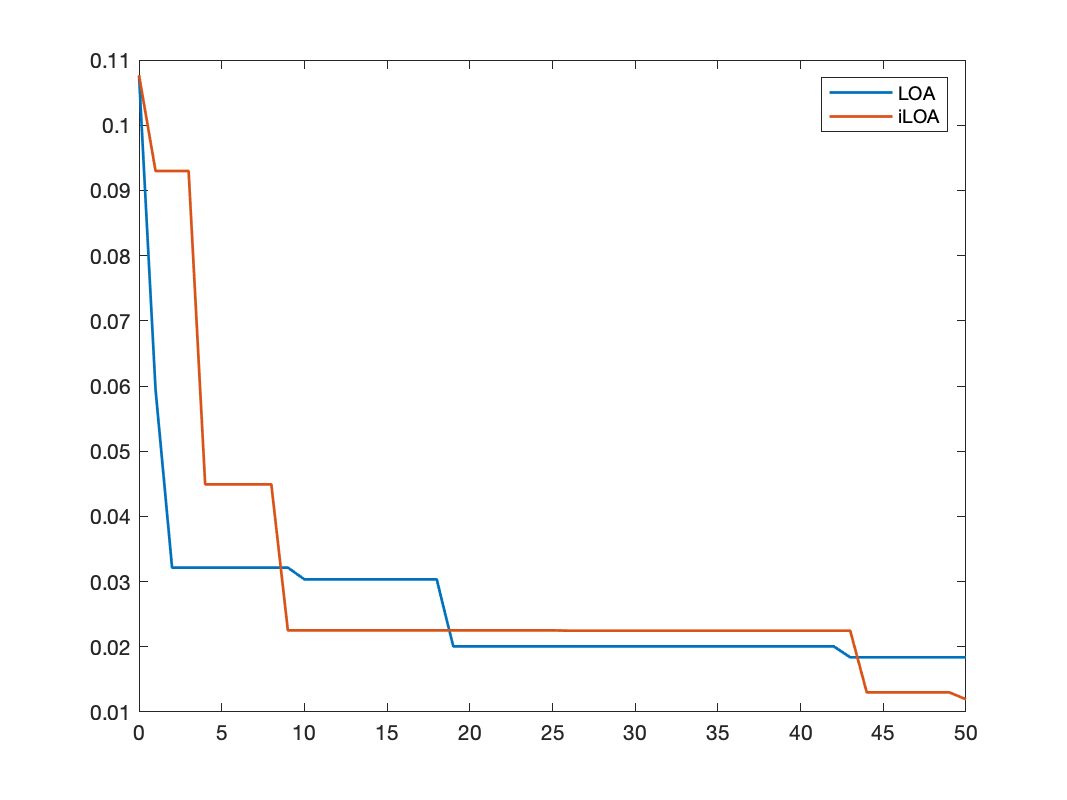
\includegraphics[width=\textwidth]{img/fits/f2/5}
    \caption{ \scriptsize Trial 5: Minimum Fitness (y) over Iterations (x)}
    \label{fig:f2-f-5}
  \end{subfigure}

  \caption{ \scriptsize LOA vs. iLOA: Griewank 2D ($f_2$)}
\end{figure}

\subsection{Rastrigin 1D}

\par Rastrigin is a non-convex function first proposed by Rastrigin as a 2-dimensional function and then generalized later on to multiple dimensions. The one-dimensional version of the function is defined by:

$$
f_3(x) = 10 + x_1^2 - 10 \cos (2 \pi x_1)
$$

It has multiple maxima and minima and its global minima is also at $x=0$.

\par Both functions are tested five times with the Rastrigin 1D function with the same starting random population and a dimensional space of [$-2\pi$, $2\pi$].

\begin{table}[ht]
\scriptsize
\begin{tabular}{l|ccccc}
\textbf{}        & \textbf{Trial 1} & \textbf{Trial 2} & \textbf{Trial 3} & \textbf{Trial 4} & \textbf{Trial 5} \\
\hline
LOA End Fitness  & 3.2384E-09       & 2.4366E-09       & 2.7632E-08       & 3.3077E-08       & 2.8756E-08       \\
LOA Evaluations  & 3401             & 3296             & 3442             & 3423             & 3379             \\
iLOA End Fitness & 1.7764E-15       & 3.5527E-15       & 3.6447E-09       & 2.2848E-10       & 2.8727E-11       \\
iLOA Evaluations & 2559             & 2631             & 2664             & 2694             & 2919
\end{tabular}
\caption{ \scriptsize LOA vs. iLOA: Rastrigin 1D ($f_3$)}
\end{table}

\begin{figure}
  \centering
  \begin{subfigure}[b]{0.4\textwidth}
    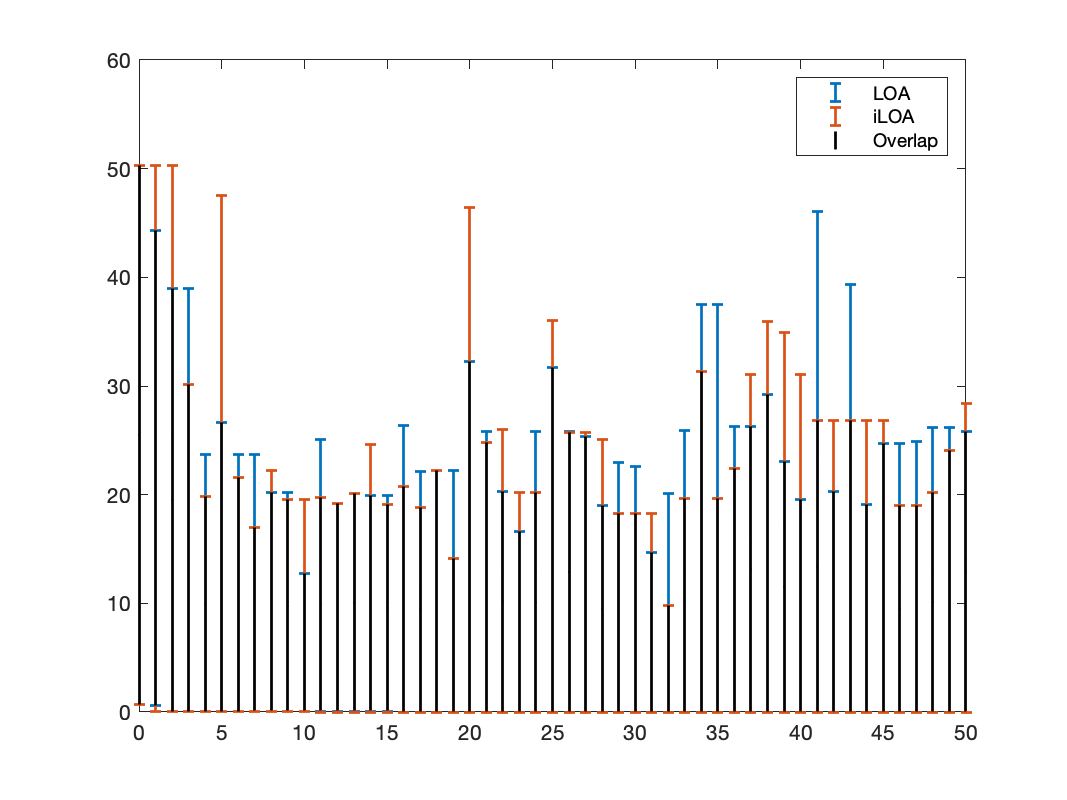
\includegraphics[width=\textwidth]{img/bars/f3/1}
    \caption{ \scriptsize Trial 1: Fitness Range (y) over Iterations (x)}
    \label{fig:f3-b-1}
  \end{subfigure}
  \begin{subfigure}[b]{0.4\textwidth}
    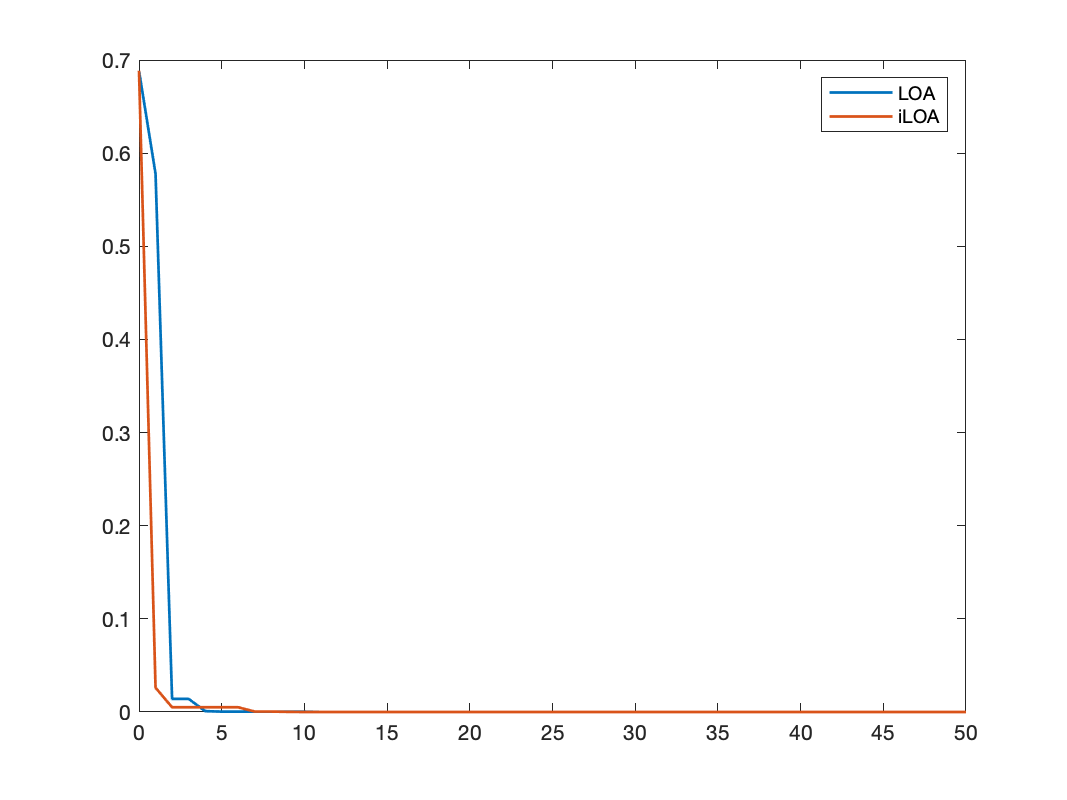
\includegraphics[width=\textwidth]{img/fits/f3/1}
    \caption{ \scriptsize Trial 1: Minimum Fitness (y) over Iterations (x)}
    \label{fig:f3-f-1}
  \end{subfigure}

  \begin{subfigure}[b]{0.4\textwidth}
    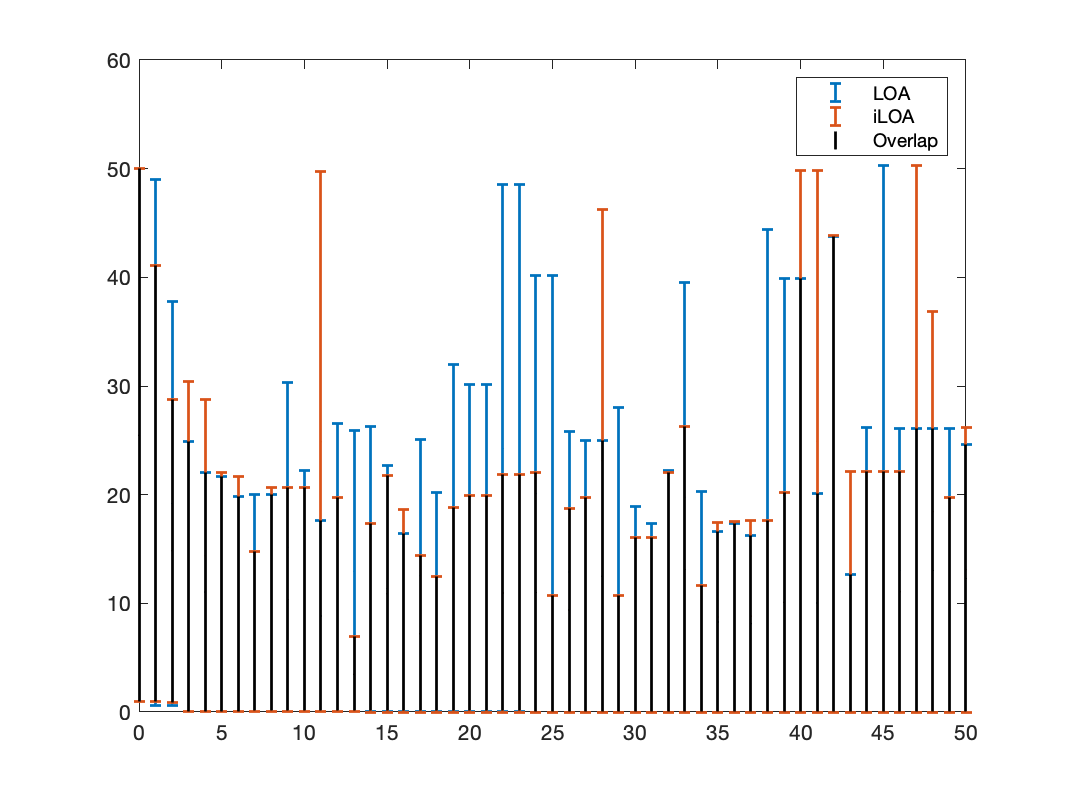
\includegraphics[width=\textwidth]{img/bars/f3/2}
    \caption{ \scriptsize Trial 2: Fitness Range (y) over Iterations (x)}
    \label{fig:f3-b-2}
  \end{subfigure}
  \begin{subfigure}[b]{0.4\textwidth}
    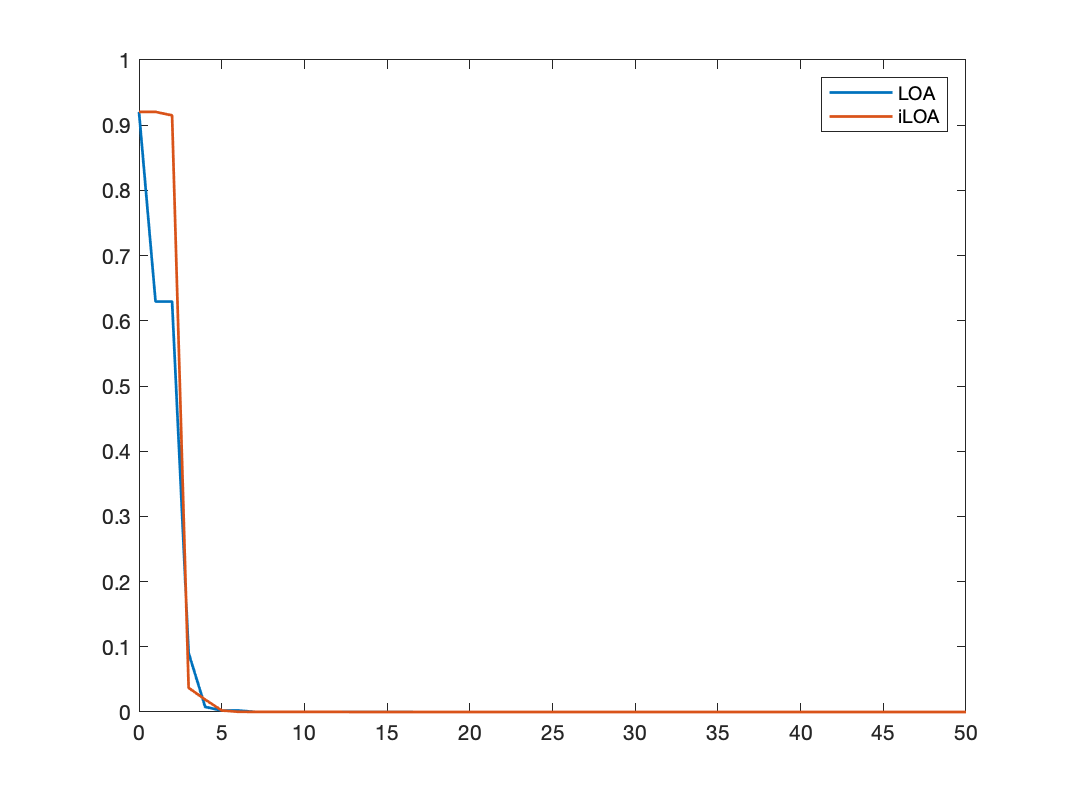
\includegraphics[width=\textwidth]{img/fits/f3/2}
    \caption{ \scriptsize Trial 2: Minimum Fitness (y) over Iterations (x)}
    \label{fig:f3-f-2}
  \end{subfigure}

  \begin{subfigure}[b]{0.4\textwidth}
    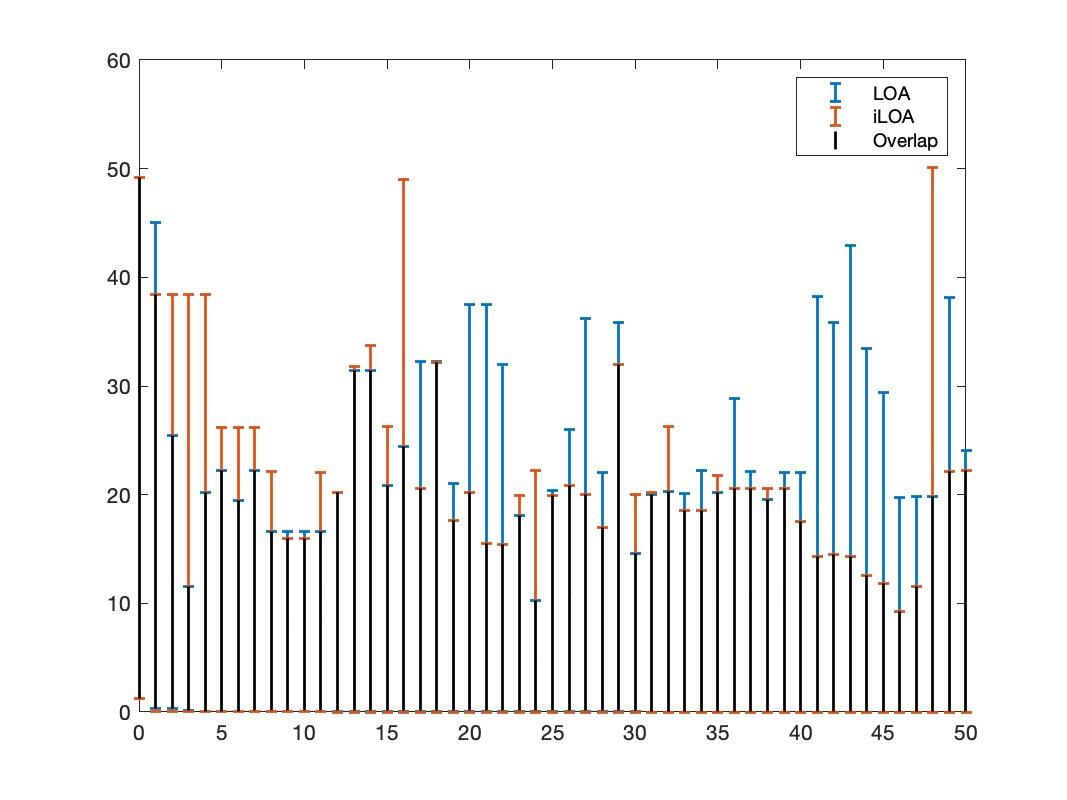
\includegraphics[width=\textwidth]{img/bars/f3/3}
    \caption{ \scriptsize Trial 3: Fitness Range (y) over Iterations (x)}
    \label{fig:f3-b-3}
  \end{subfigure}
  \begin{subfigure}[b]{0.4\textwidth}
    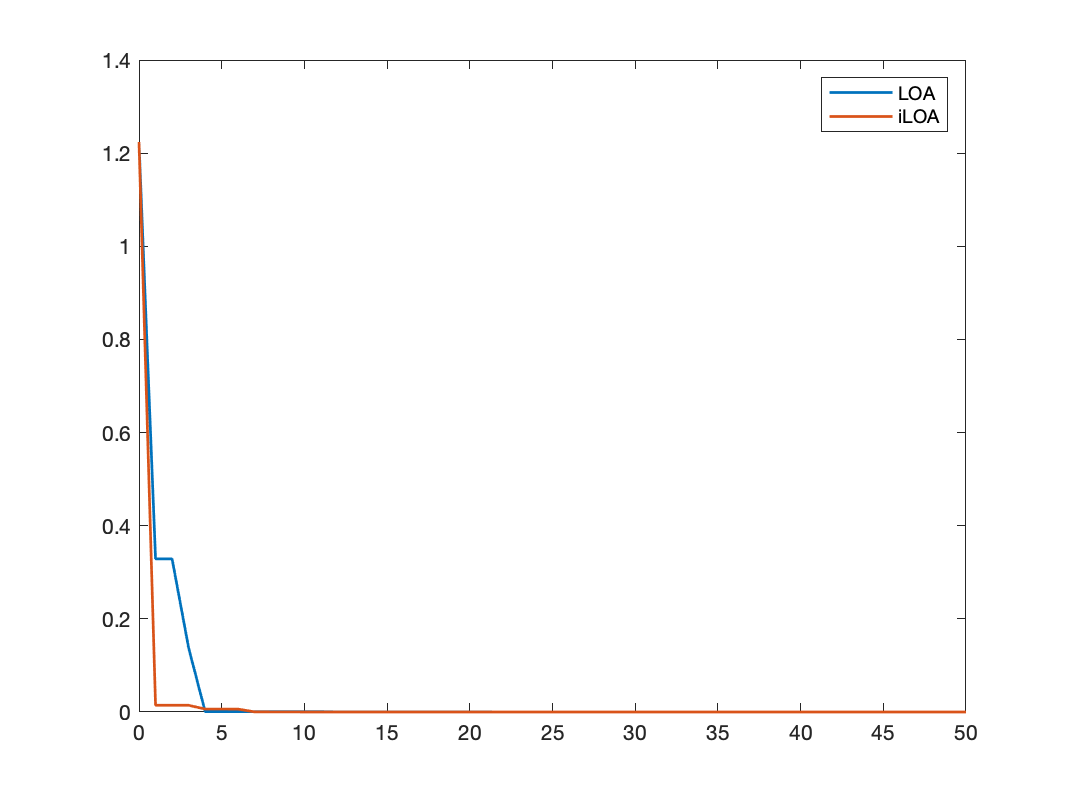
\includegraphics[width=\textwidth]{img/fits/f3/3}
    \caption{ \scriptsize Trial 3: Minimum Fitness (y) over Iterations (x)}
    \label{fig:f3-f-3}
  \end{subfigure}

  \begin{subfigure}[b]{0.4\textwidth}
    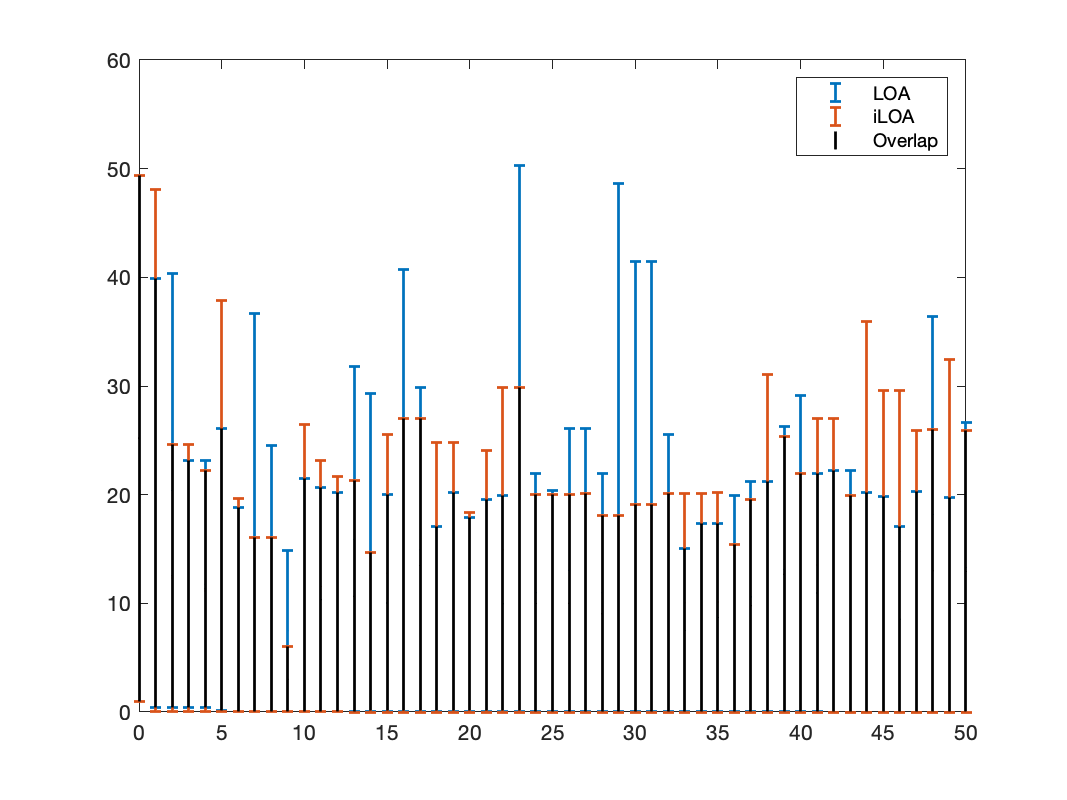
\includegraphics[width=\textwidth]{img/bars/f3/4}
    \caption{ \scriptsize Trial 4: Fitness Range (y) over Iterations (x)}
    \label{fig:f3-b-4}
  \end{subfigure}
  \begin{subfigure}[b]{0.4\textwidth}
    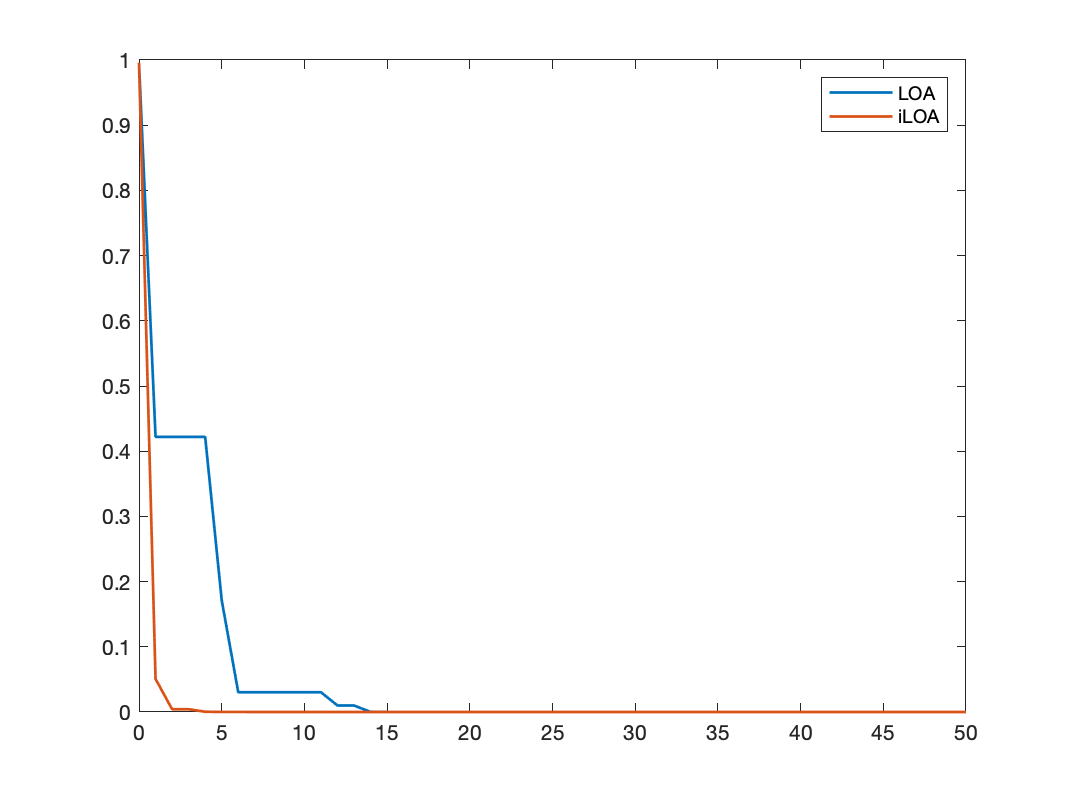
\includegraphics[width=\textwidth]{img/fits/f3/4}
    \caption{ \scriptsize Trial 4: Minimum Fitness (y) over Iterations (x)}
    \label{fig:f3-f-4}
  \end{subfigure}

  \begin{subfigure}[b]{0.4\textwidth}
    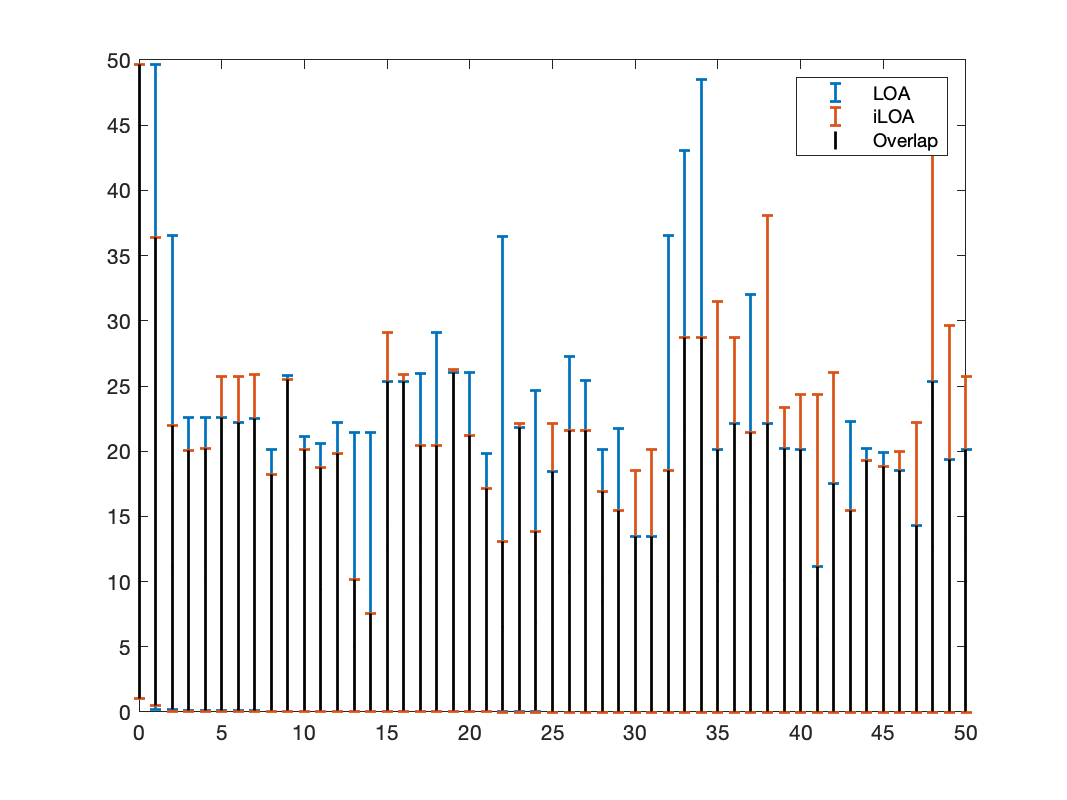
\includegraphics[width=\textwidth]{img/bars/f3/5}
    \caption{ \scriptsize Trial 5: Fitness Range (y) over Iterations (x)}
    \label{fig:f3-b-5}
  \end{subfigure}
  \begin{subfigure}[b]{0.4\textwidth}
    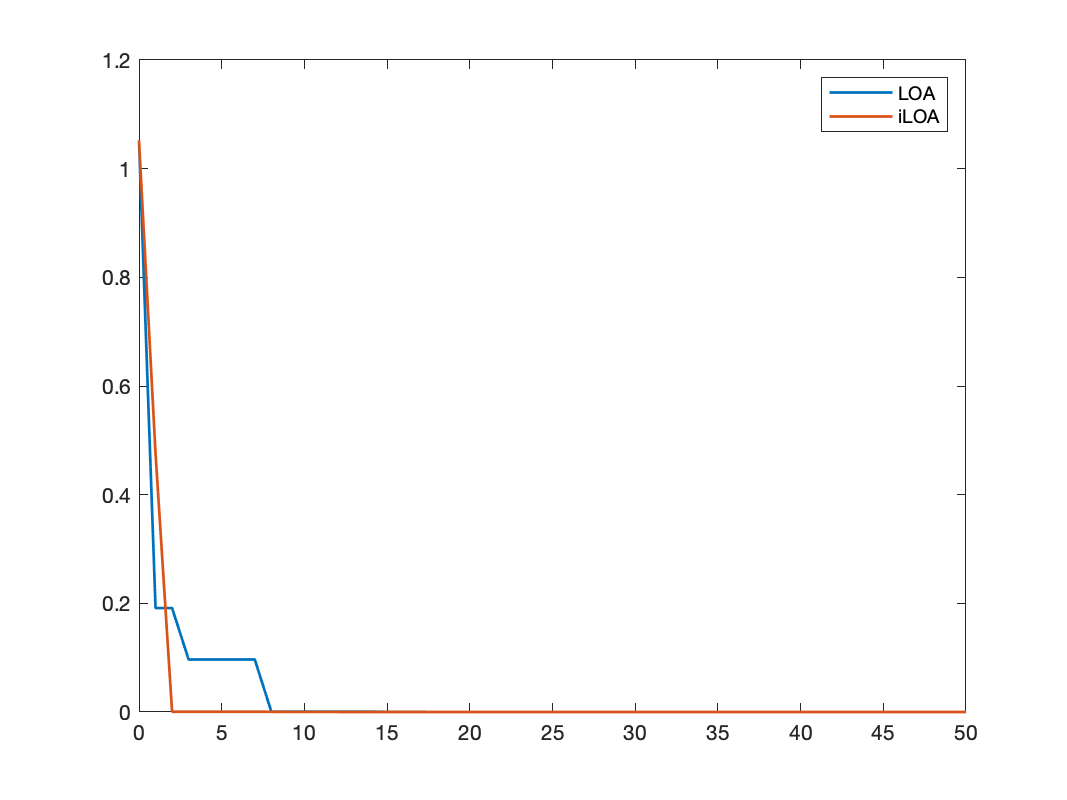
\includegraphics[width=\textwidth]{img/fits/f3/5}
    \caption{ \scriptsize Trial 5: Minimum Fitness (y) over Iterations (x)}
    \label{fig:f3-f-5}
  \end{subfigure}

  \caption{ \scriptsize LOA vs. iLOA: Rastrigin 1D ($f_3$)}
\end{figure}

\subsection{Rastrigin 2D}

\par Rastrigin is a non-convex function first proposed by Rastrigin as a 2-dimensional function and then generalized later on to multiple dimensions. The function is defined by:

$$
f_4(x) = 20 + x_1^2 - 10 \cos (2 \pi x_1) + x_2^2 - 10 \cos (2 \pi x_2)
$$

It has multiple maxima and minima and its global minima is also at $x=0$.

\par Both functions are tested five times with the Rastrigin 2D function with the same starting random population and a dimensional space of [$-2\pi$, $2\pi$].

\begin{table}[ht]
\scriptsize
\begin{tabular}{l|ccccc}
\textbf{}        & \textbf{Trial 1} & \textbf{Trial 2} & \textbf{Trial 3} & \textbf{Trial 4} & \textbf{Trial 5} \\
\hline
LOA End Fitness  & 0.083296         & 0.022199         & 0.001943         & 0.0015496        & 0.30548          \\
LOA Evaluations  & 3314             & 3513             & 3443             & 3536             & 3496             \\
iLOA End Fitness & 0.00022399       & 0.0015992        & 0.0012708        & 0.40278          & 3.1202E-05       \\
iLOA Evaluations & 2811             & 2767             & 2711             & 2743             & 2894
\end{tabular}
\caption{ \scriptsize LOA vs. iLOA: Rastrigin 2D ($f_4$)}
\end{table}

\begin{figure}
  \centering
  \begin{subfigure}[b]{0.4\textwidth}
    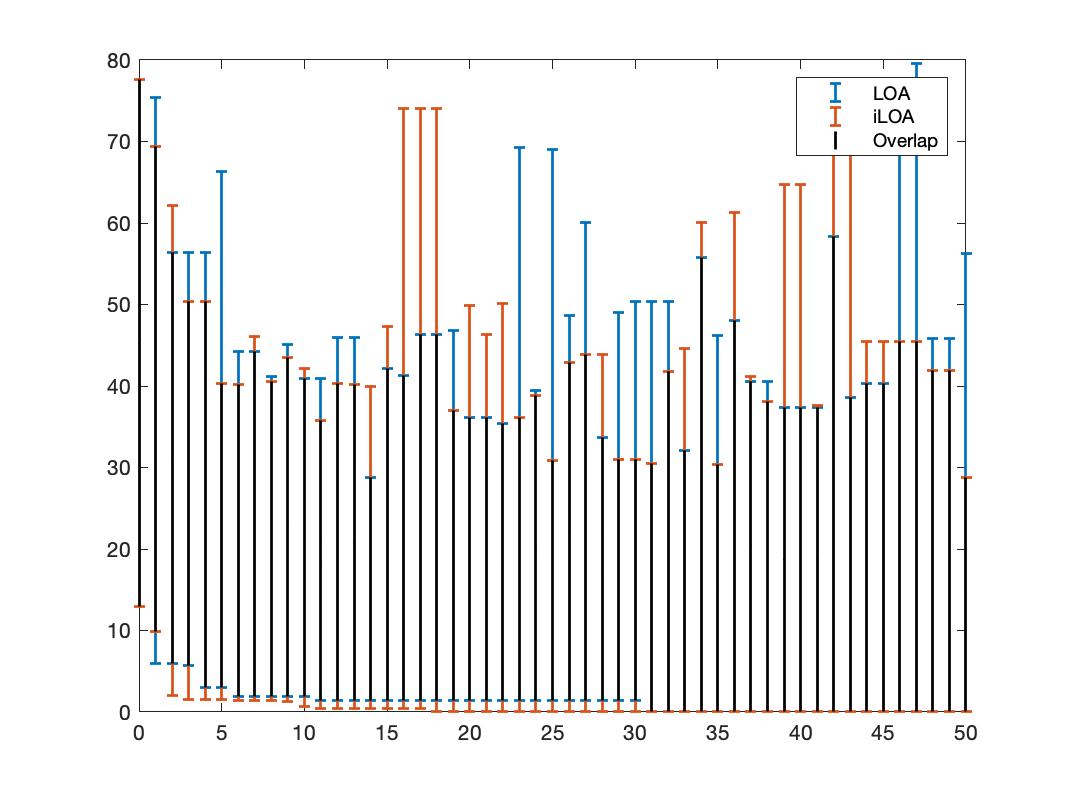
\includegraphics[width=\textwidth]{img/bars/f4/1}
    \caption{ \scriptsize Trial 1: Fitness Range (y) over Iterations (x)}
    \label{fig:f4-b-1}
  \end{subfigure}
  \begin{subfigure}[b]{0.4\textwidth}
    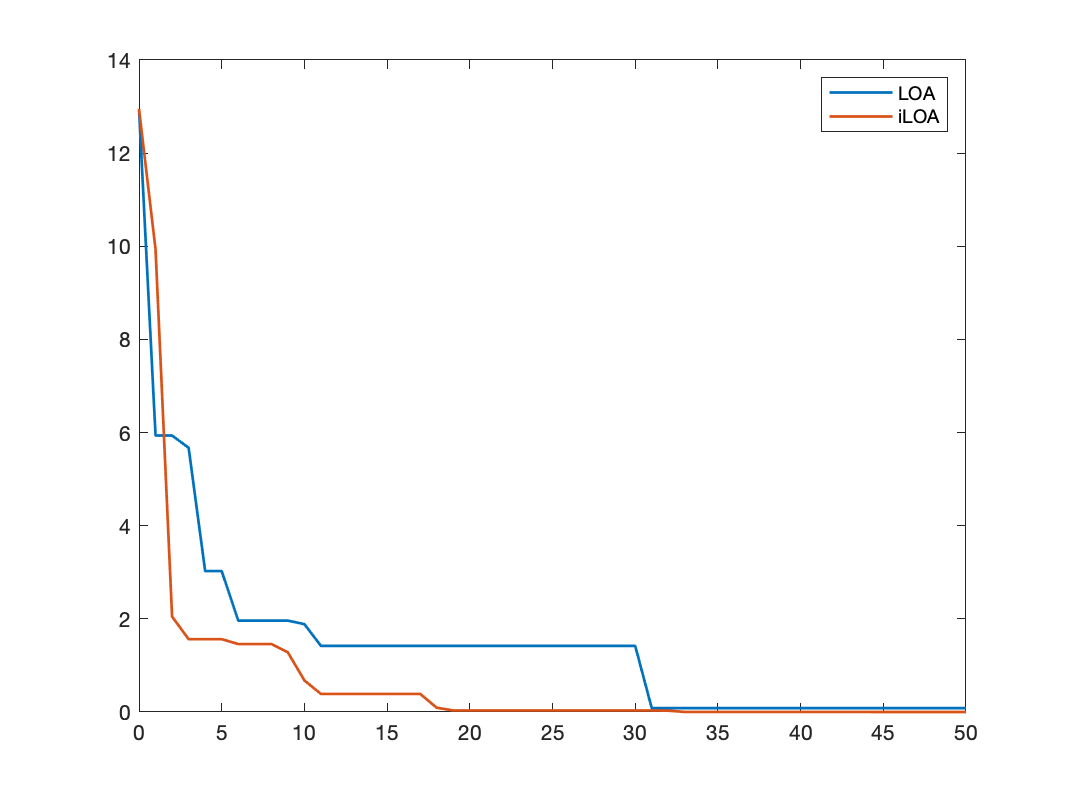
\includegraphics[width=\textwidth]{img/fits/f4/1}
    \caption{ \scriptsize Trial 1: Minimum Fitness (y) over Iterations (x)}
    \label{fig:f4-f-1}
  \end{subfigure}

  \begin{subfigure}[b]{0.4\textwidth}
    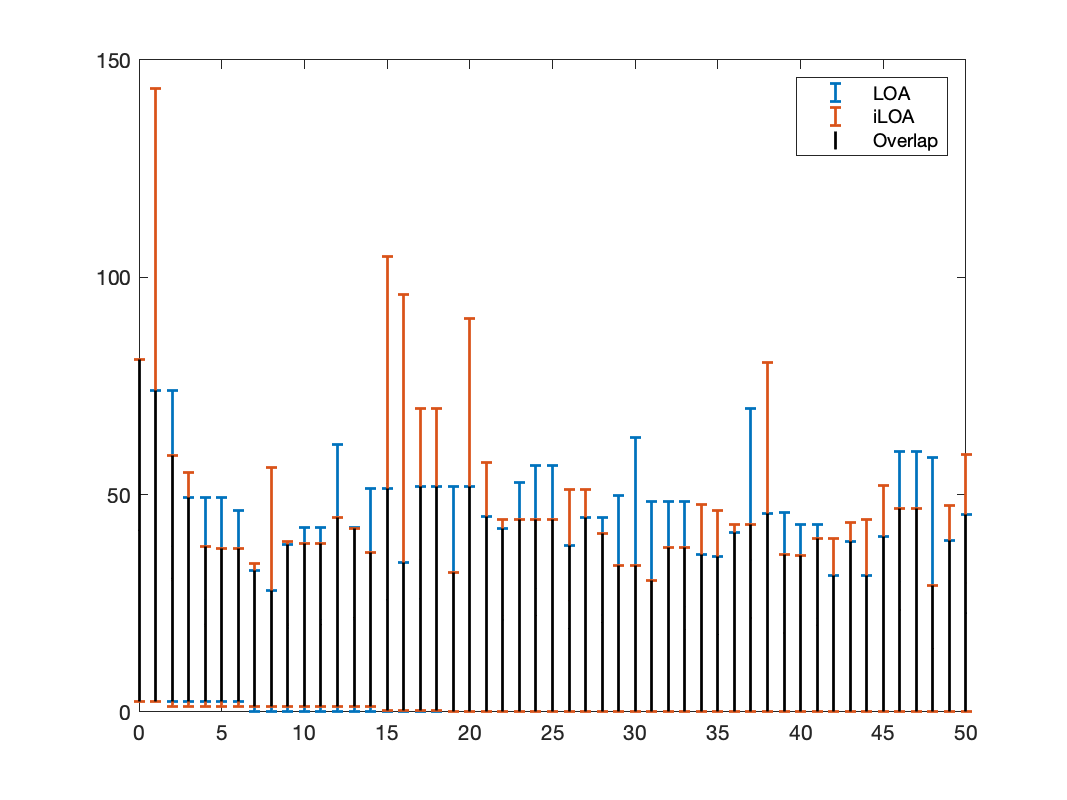
\includegraphics[width=\textwidth]{img/bars/f4/2}
    \caption{ \scriptsize Trial 2: Fitness Range (y) over Iterations (x)}
    \label{fig:f4-b-2}
  \end{subfigure}
  \begin{subfigure}[b]{0.4\textwidth}
    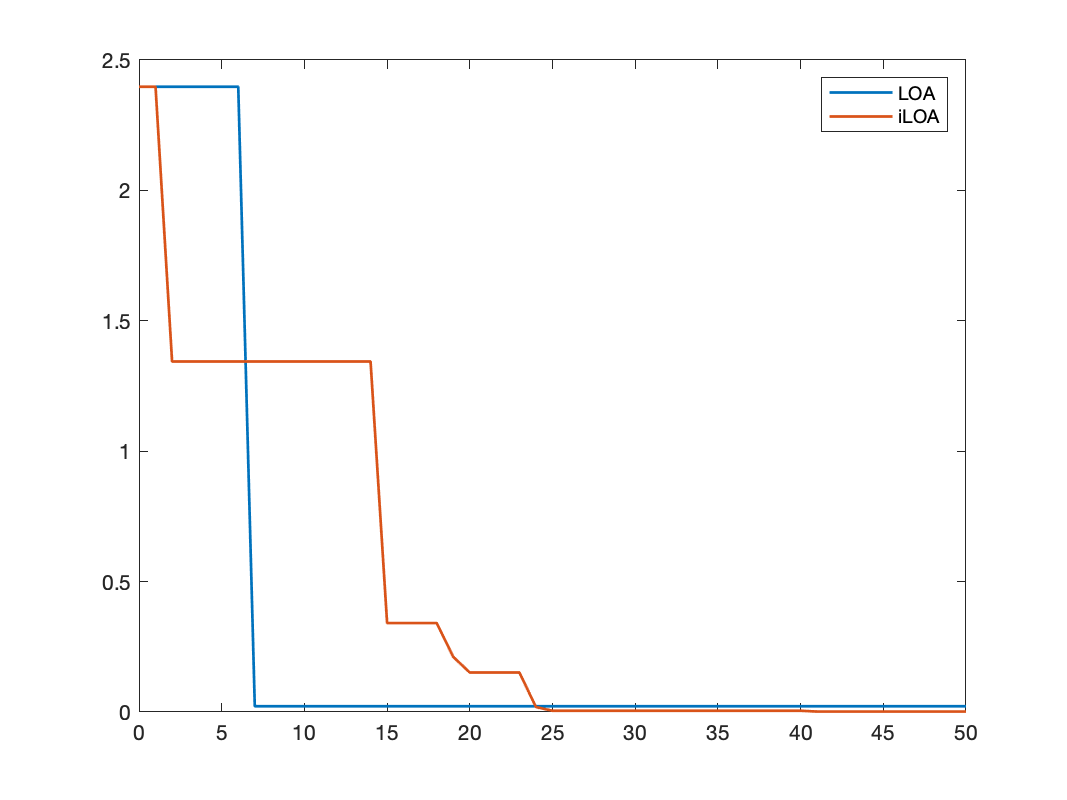
\includegraphics[width=\textwidth]{img/fits/f4/2}
    \caption{ \scriptsize Trial 2: Minimum Fitness (y) over Iterations (x)}
    \label{fig:f4-f-2}
  \end{subfigure}

  \begin{subfigure}[b]{0.4\textwidth}
    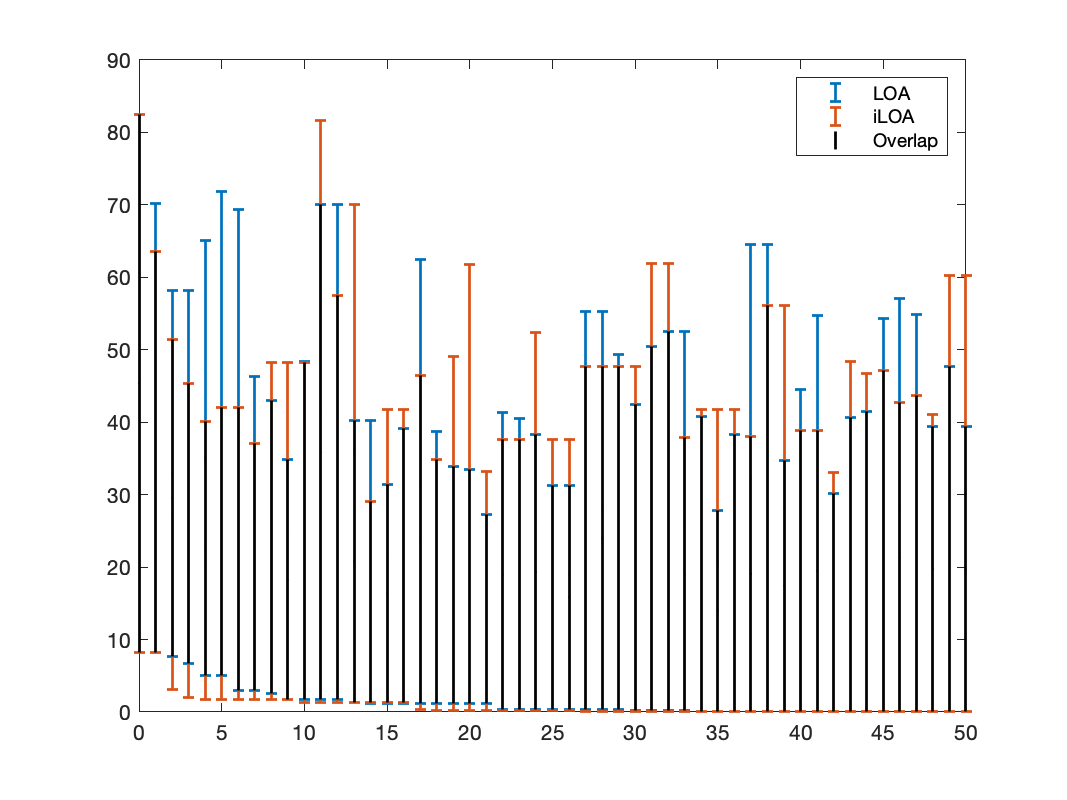
\includegraphics[width=\textwidth]{img/bars/f4/3}
    \caption{ \scriptsize Trial 3: Fitness Range (y) over Iterations (x)}
    \label{fig:f4-b-3}
  \end{subfigure}
  \begin{subfigure}[b]{0.4\textwidth}
    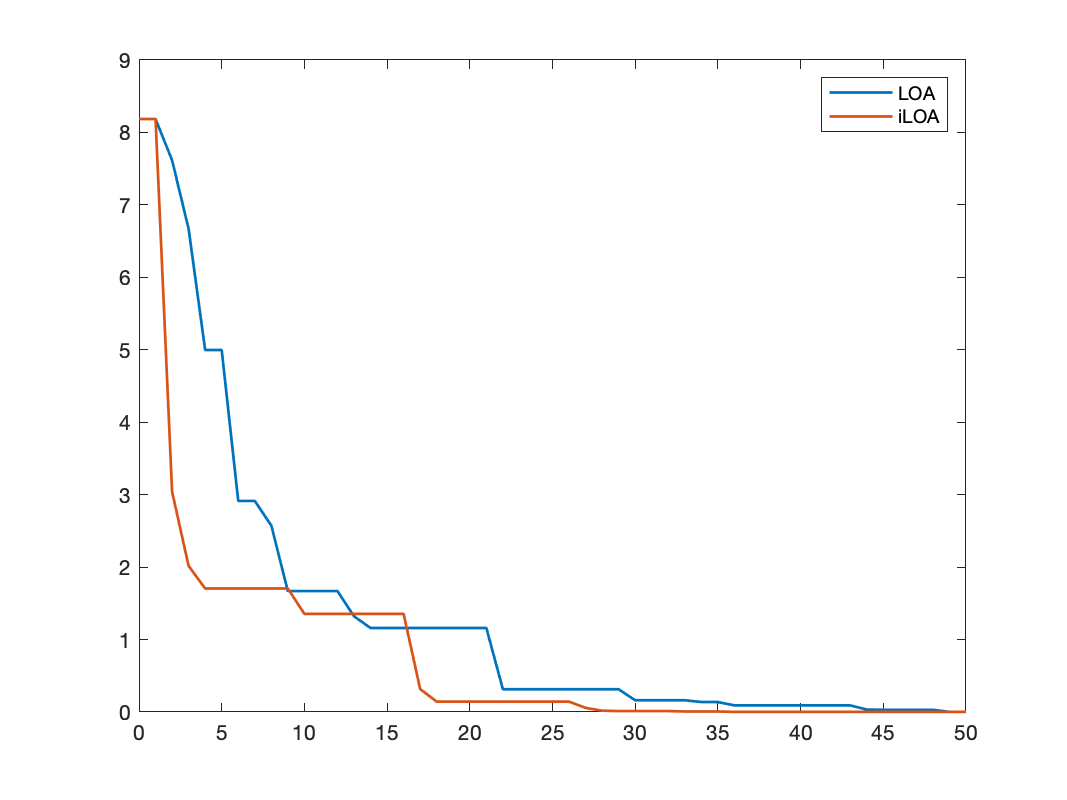
\includegraphics[width=\textwidth]{img/fits/f4/3}
    \caption{ \scriptsize Trial 3: Minimum Fitness (y) over Iterations (x)}
    \label{fig:f4-f-3}
  \end{subfigure}

  \begin{subfigure}[b]{0.4\textwidth}
    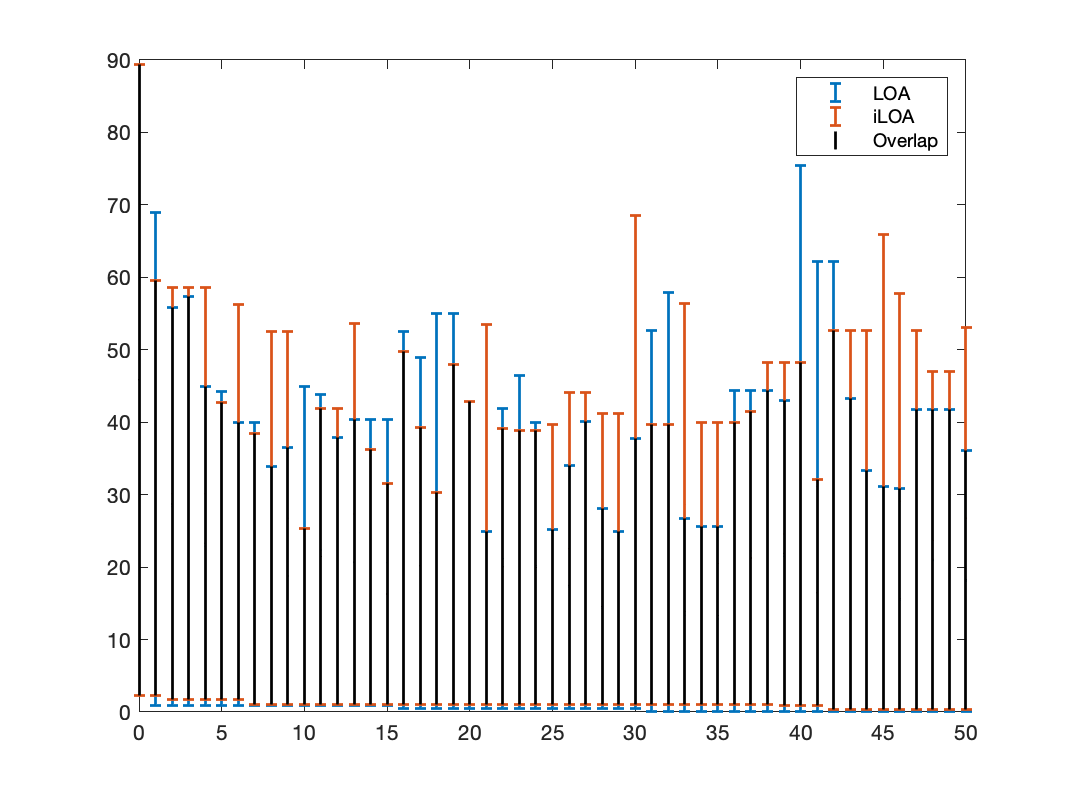
\includegraphics[width=\textwidth]{img/bars/f4/4}
    \caption{ \scriptsize Trial 4: Fitness Range (y) over Iterations (x)}
    \label{fig:f4-b-4}
  \end{subfigure}
  \begin{subfigure}[b]{0.4\textwidth}
    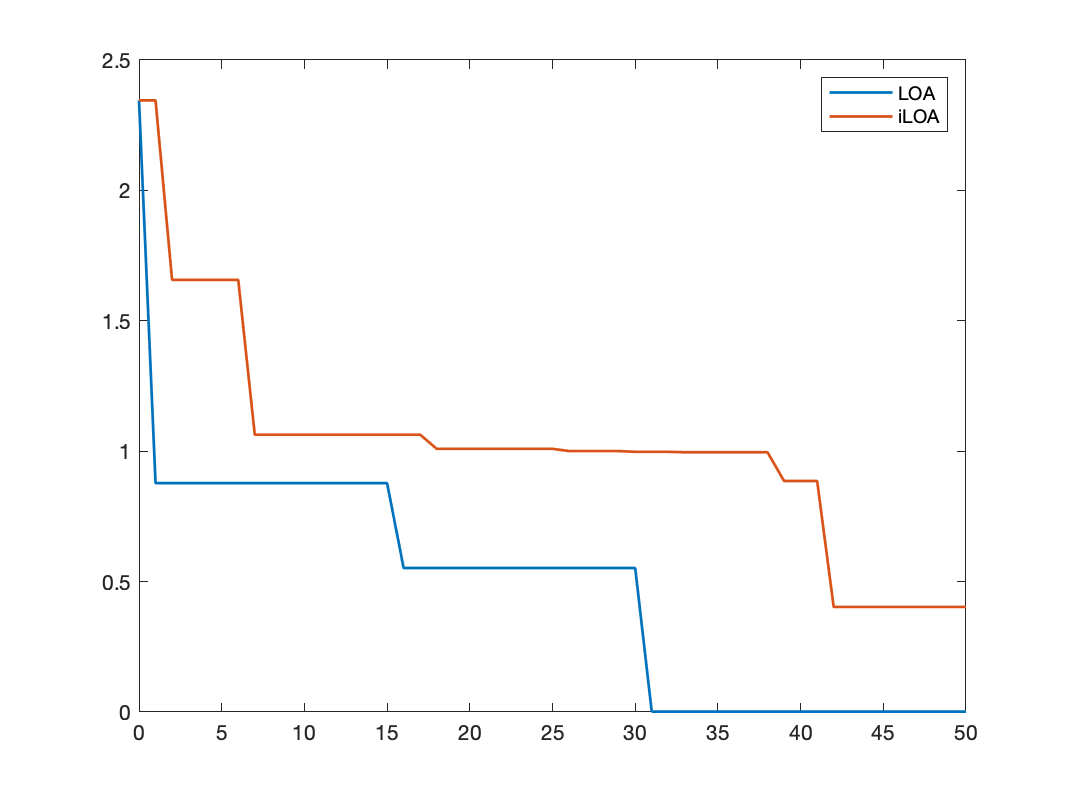
\includegraphics[width=\textwidth]{img/fits/f4/4}
    \caption{ \scriptsize Trial 4: Minimum Fitness (y) over Iterations (x)}
    \label{fig:f4-f-4}
  \end{subfigure}

  \begin{subfigure}[b]{0.4\textwidth}
    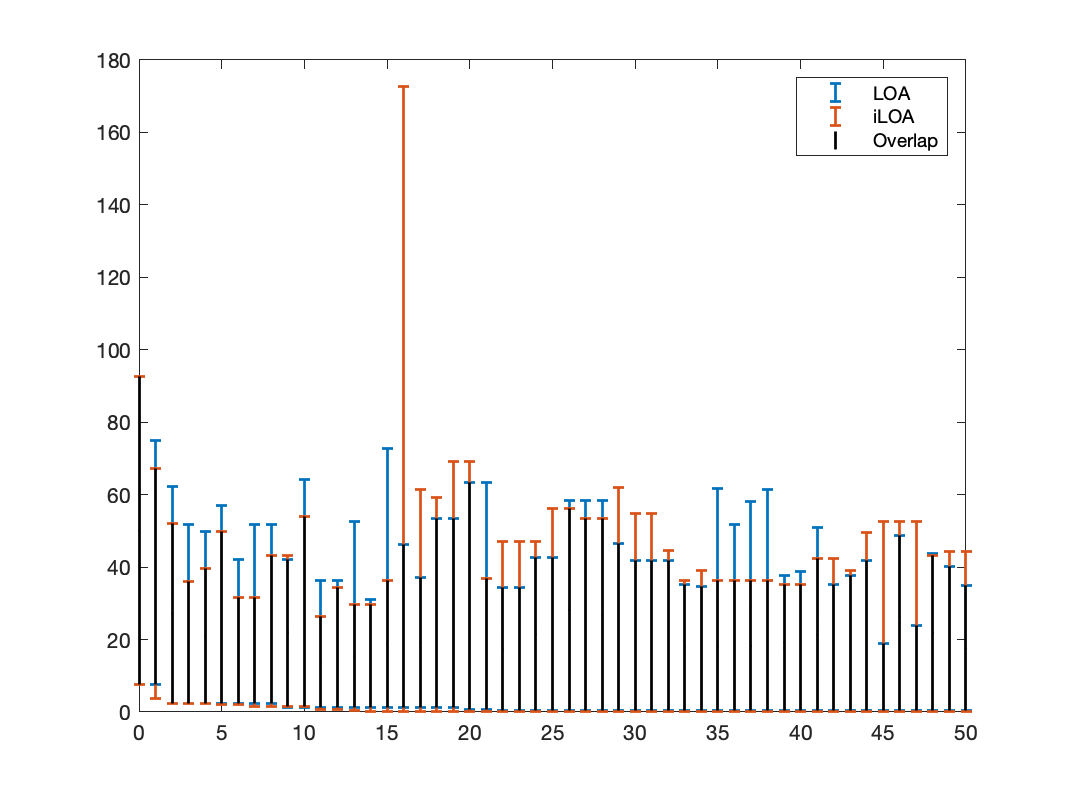
\includegraphics[width=\textwidth]{img/bars/f4/5}
    \caption{ \scriptsize Trial 5: Fitness Range (y) over Iterations (x)}
    \label{fig:f4-b-5}
  \end{subfigure}
  \begin{subfigure}[b]{0.4\textwidth}
    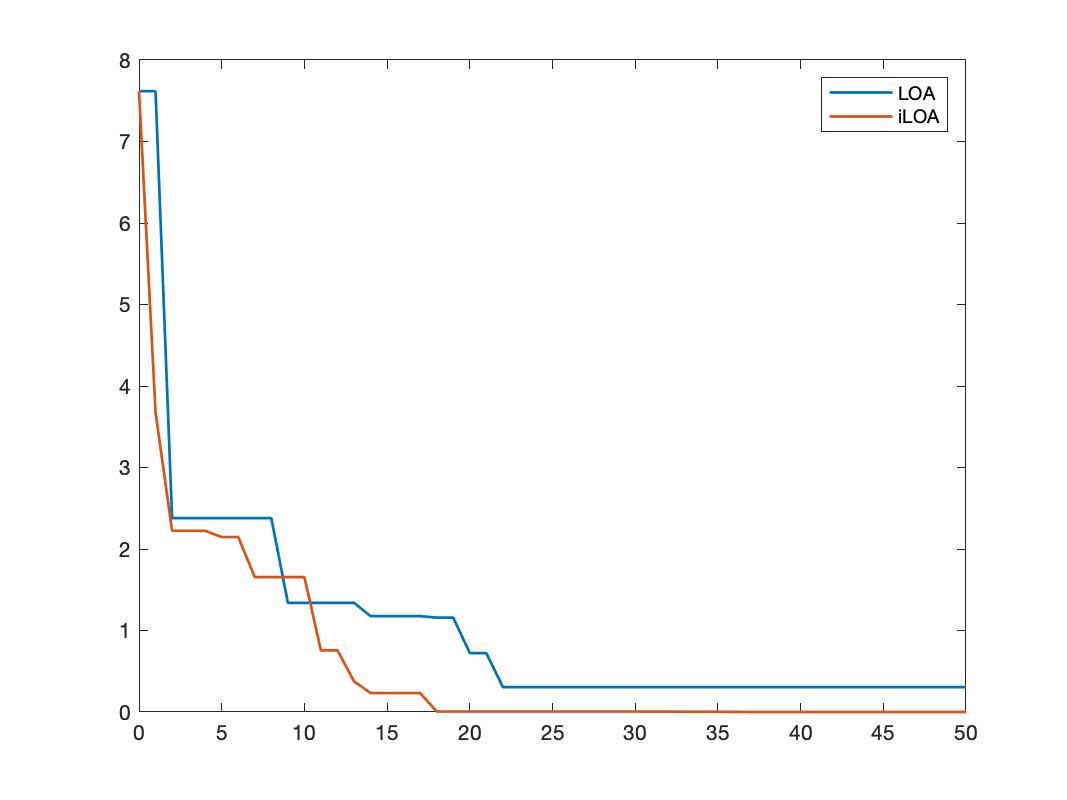
\includegraphics[width=\textwidth]{img/fits/f4/5}
    \caption{ \scriptsize Trial 5: Minimum Fitness (y) over Iterations (x)}
    \label{fig:f4-f-5}
  \end{subfigure}

  \caption{ \scriptsize LOA vs. iLOA: Rastrigin 2D ($f_4$)}
\end{figure}

\subsection{Rosenbrock 2D}

\par Rastrigin is a non-convex function proposed by Howard H. Rosenbrock as a 2-dimensional function for testing optimization and then generalized later on to multiple dimensions. The function is defined by:

$$
f_5(x) = (a-x_1)^2+b(x_2-x_1^2)^2
$$

where $a=1$ and $b=100$. It has multiple maxima and minima and its global minima is at $x=<a,a^2>$ or $<1,1>$.

\par Both functions are tested five times with the Rosenbrock 2D function with the same starting random population and a dimensional space of [$-5$, $5$].

\begin{table}[ht]
\scriptsize
\begin{tabular}{l|ccccc}
\textbf{}        & \textbf{Trial 1} & \textbf{Trial 2} & \textbf{Trial 3} & \textbf{Trial 4} & \textbf{Trial 5} \\
\hline
LOA End Fitness  & 0.0049932        & 0.00015138       & 0.002005         & 0.0018016        & 0.000050672          \\
LOA Evaluations  & 3540             & 3277             & 3263             & 3260             & 3284             \\
iLOA End Fitness & 0.015473         & 0.00066979       & 0.00023044       & 0.000033068      & 5.8865E-06       \\
iLOA Evaluations & 2688             & 2873             & 2786             & 2694             & 2858
\end{tabular}
\caption{ \scriptsize LOA vs. iLOA: Rosenbrock 2D ($f_5$)}
\end{table}

\begin{figure}
  \centering
  \begin{subfigure}[b]{0.4\textwidth}
    \includegraphics[width=\textwidth]{img/bars/f5/1}
    \caption{ \scriptsize Trial 1: Fitness Range (y) over Iterations (x)}
    \label{fig:f5-b-1}
  \end{subfigure}
  \begin{subfigure}[b]{0.4\textwidth}
    \includegraphics[width=\textwidth]{img/fits/f5/1}
    \caption{ \scriptsize Trial 1: Minimum Fitness (y) over Iterations (x)}
    \label{fig:f5-f-1}
  \end{subfigure}

  \begin{subfigure}[b]{0.4\textwidth}
    \includegraphics[width=\textwidth]{img/bars/f5/2}
    \caption{ \scriptsize Trial 2: Fitness Range (y) over Iterations (x)}
    \label{fig:f5-b-2}
  \end{subfigure}
  \begin{subfigure}[b]{0.4\textwidth}
    \includegraphics[width=\textwidth]{img/fits/f5/2}
    \caption{ \scriptsize Trial 2: Minimum Fitness (y) over Iterations (x)}
    \label{fig:f5-f-2}
  \end{subfigure}

  \begin{subfigure}[b]{0.4\textwidth}
    \includegraphics[width=\textwidth]{img/bars/f5/3}
    \caption{ \scriptsize Trial 3: Fitness Range (y) over Iterations (x)}
    \label{fig:f5-b-3}
  \end{subfigure}
  \begin{subfigure}[b]{0.4\textwidth}
    \includegraphics[width=\textwidth]{img/fits/f5/3}
    \caption{ \scriptsize Trial 3: Minimum Fitness (y) over Iterations (x)}
    \label{fig:f5-f-3}
  \end{subfigure}

  \begin{subfigure}[b]{0.4\textwidth}
    \includegraphics[width=\textwidth]{img/bars/f5/4}
    \caption{ \scriptsize Trial 4: Fitness Range (y) over Iterations (x)}
    \label{fig:f5-b-4}
  \end{subfigure}
  \begin{subfigure}[b]{0.4\textwidth}
    \includegraphics[width=\textwidth]{img/fits/f5/4}
    \caption{ \scriptsize Trial 4: Minimum Fitness (y) over Iterations (x)}
    \label{fig:f5-f-4}
  \end{subfigure}

  \begin{subfigure}[b]{0.4\textwidth}
    \includegraphics[width=\textwidth]{img/bars/f5/5}
    \caption{ \scriptsize Trial 5: Fitness Range (y) over Iterations (x)}
    \label{fig:f5-b-5}
  \end{subfigure}
  \begin{subfigure}[b]{0.4\textwidth}
    \includegraphics[width=\textwidth]{img/fits/f5/5}
    \caption{ \scriptsize Trial 5: Minimum Fitness (y) over Iterations (x)}
    \label{fig:f5-f-5}
  \end{subfigure}

  \caption{ \scriptsize LOA vs. iLOA: Rosenbrock 2D ($f_5$)}
\end{figure}

\section{Parameter Testing for iLOA}

\par Parameter tests are done for each of the aforementioned functions by performing an exhaustive search on the following parameter points:

\fbox{\begin{minipage}{0.9\textwidth}
\scriptsize
\textbf{Nomad Percentage (\%N)} = \{0.2, 0.4, 0.6, 0.8\} \\
\textbf{Roaming Percentage (\%R)} = \{0.2, 0.4, 0.6, 0.8\} \\
\textbf{Sex Percentage (\%S)} = \{0.2, 0.4, 0.6, 0.8\} \\
\textbf{Mating Rate (\%Ma)} = \{0.3, 0.6\} \\
\textbf{Mutation Probability} = \{0.2, 0.4, 0.6, 0.8\} \\
\textbf{Immigration Rate} = \{0.2, 0.4, 0.6, 0.8\} \\
\textbf{Percent Group Influence} = \{0.2, 0.4, 0.6, 0.8\} \\
\textbf{Ranked Selection Pressure} = \{2, 3\} \\
\textbf{Near to Best Random Pressure} = \{2, 3\}
\end{minipage}}

\par Each of the functions is run using every possible set of parameters using the above parameter points and their outputs recorded so that the best parameter set is found.

\par Each function is tested against iLOA with every parameter set running 5 times each for redundancy. The iterations are limited to 30, includes 4 prides and a population of 50 for the parameters.

\subsection{Test Limitations}
\par The platform used for both the algorithm code and parameter tester, MATLAB, has its own limitations of number representation when representing float values of numbers with decimal places with more than 16 binary digits (values smaller than $2^{-16}$). Now, all of one-dimensional Griewank, one-dimensional Rastrigin and two-dimensional Rastrigin has encountered this limitations such that some of their fitness data represented results being zero upon data collection.

\par Instead of using the mentioned functions, the three-dimensional Griewank, three-dimensional Rastrigin and four-dimensional Rastrigin functions are used. These functions not only are similar to their replaced counterparts but have larger search space than their counterparts.

\section{Rastrigin Function}

\par The Rastrigin function, as defined in the earlier sections, is a non-convex function with a multi-dimensional form:
$$
f(x) = A n + \sum_{i=1}^n \left[x_i^2 - A\cos(2 \pi x_i)\right]
$$

\subsection{Three-Dimensional Rastrigin Function}

\par The parameter set found to have the best average fitness for the three-dimensional Rastrigin is the parameters

\fbox{\begin{minipage}{0.9\textwidth}
\scriptsize
Nomad Percentage (\%N) = 0.2 \\
Roaming Percentage (\%R) = 0.8 \\
Sex Percentage (\%S) = 0.2 \\
Mating Rate (\%Ma) = 0.6 \\
Mutation Probability = 0.8 \\
Immigration Rate = 0.8 \\
Percent Group Influence = 0.6 \\
Ranked Selection Pressure = 2 \\
Near to Best Random Pressure = 3 \\
\textbf{Parameter Set Average Fitness: 2.8400e-15}
\end{minipage}}

\subsection{Four-Dimensional Rastrigin Function}

\par The parameter set found to have the best average fitness for the four-dimensional Rastrigin is the parameters

\fbox{\begin{minipage}{0.9\textwidth}
\scriptsize
Nomad Percentage (\%N) = 0.4 \\
Roaming Percentage (\%R) = 0.8 \\
Sex Percentage (\%S) = 0.8 \\
Mating Rate (\%Ma) = 0.6 \\
Mutation Probability = 0.6 \\
Immigration Rate = 0.6 \\
Percent Group Influence = 0.8 \\
Ranked Selection Pressure = 2 \\
Near to Best Random Pressure = 3 \\
\textbf{Parameter Set Average Fitness: 0.1499}
\end{minipage}}

\par While the three-dimensional function parameters has a low sex percentage (Percent females in prides, Percent males in nomads), the four-dimensional function paramaters does the opposite with a high sex percentage while balancing it with an increased nomad percentage. The four-dimensional function parameters also tries to decrease its mutation probability to focus on not losing the current solutions in the larger search space and improve those solutions for better ones. Also since the Rastrigin function has many optimas, the ``Near to Best'' Random Pressure is increased such that the solutions generated are near each other such that those new solutions likely would be generated next to an optima.

\section{Griewank Function}

\subsection{Two-Dimensional Griewank}

4.0000    0.2000    0.8000    0.2000    0.6000    0.8000    0.2000    0.8000    1.0000    2.0000    2.0000

1.1100e-16

\subsection{Three-Dimensional Griewank}

4.0000    0.2000    0.6000    0.2000    0.3000    0.4000    0.8000    0.2000    1.0000    3.0000    3.0000

0.0064
 
\section{Rosenbrock Function}

\par The parameter set found to have the best average fitness for the Rosenbrock Function are the parameters

\fbox{\begin{minipage}{0.9\textwidth}
\scriptsize
Nomad Percentage (\%N) = 0.2 \\
Roaming Percentage (\%R) = 0.8 \\
Sex Percentage (\%S) = 0.6 \\
Mating Rate (\%Ma) = 0.6 \\
Mutation Probability = 0.2 \\
Immigration Rate = 0.8 \\
Percent Group Influence = 0.8 \\
Ranked Selection Pressure = 2 \\
Near to Best Random Pressure = 3 \\
\textbf{Parameter Set Average Fitness: 3.3754e-14}
\end{minipage}}

\par The above parameter set focuses on more information sharing between points and less random generation of solutions. While there is a high roaming percentage, the nomads for this parameter set are minimal. The high immigration rate and percent group influence increases the chances for prides to exchange information within and to other prides and the minimal mutation probability decreases the randomness of solutions.

\par Since the Rosenbrock function's surface has a ridge where the fitness tends to get better, this parameter set gives the algorithm a chance to focus on not losing more solutions and focus on improving the solutions that get to the narrow window of high fitness that is found on the ridge of the Rosenbrock function's surface while also influencing other solutions to reach the area.

\subsection{Parameter Testing Conclusion}
\par There are different parameter sets that perform better for each function. This only implies that the No Free Lunch Theorem is at work. Having different parameter sets makes each instance of iLOA algorithm different from other instances with a different parameter set. Each function works best with a certain instance of iLOA with a certain parameter set.

\par The previous test proves that smaller search spaces tends to have a higher randomability in its parameter set since smaller spaces are easy to scan through for the best points and that larger search spaces decrease its randomability since larger spaces are harder to scan through such that improving on the best solutions so far is more convenient.

\par The parameter set also depends on how many optima that can be found from the functions. High count optima functions like Rastrigin tend to favor randomability more while low count optima functions like Rosenbrock tend to favor selection imrpovement more over randomability.

\par Taking the most common best parameter points that were used by the functions, the most common parameter setup for iLOA is:

\fbox{\begin{minipage}{0.9\textwidth}
\scriptsize
Nomad Percentage (\%N) = 0.2 (ave 0.24) \\
Roaming Percentage (\%R) = 0.8 (ave 0.76) \\
Sex Percentage (\%S) = 0.4 (ave 0.4) \\
Mating Rate (\%Ma) = 0.5 (ave 0.54) \\
Mutation Probability = 0.6 (ave 0.56) \\
Immigration Rate = 0.6 (ave 0.64) \\
Percent Group Influence = 0.6 (ave 0.64) \\
Ranked Selection Pressure = 2 (ave 2.3) \\
Near to Best Random Pressure = 3 (ave 2.8)
\end{minipage}}

\par Since most of the functions used in the tests is of type high count optima, the above parameter set is biased to high count optima functions.


%----------------------------------------------------------------------------------------
%	BIBLIOGRAPHY
%----------------------------------------------------------------------------------------

\bibliographystyle{plain}

\bibliography{refs}

%----------------------------------------------------------------------------------------

\end{document}
